% $Author: oscar $
% $Date: 2009-09-15 16:53:48 +0200 (Tue, 15 Sep 2009) $
% $Revision: 29111 $
%=================================================================
\ifx\wholebook\relax\else
% --------------------------------------------
% Lulu:
	\documentclass[a4paper,10pt,twoside]{book}
	\usepackage[
		papersize={6.13in,9.21in},
		hmargin={.815in,.815in},
		vmargin={.98in,.98in},
		ignoreheadfoot
	]{geometry}
	\usepackage[hangul]{kotex}
	% $Author: oscar $
% $Date: 2009-09-13 20:58:29 +0200 (Sun, 13 Sep 2009) $
% $Revision: 29070 $
%=============================================================
% NB: documentclass must be set in main document.
% Allows book to be generated in multiple formats.
%=============================================================
%:Packages
\usepackage[T1]{fontenc}  %%%%%really important to get the code directly in the text!
\usepackage{palatino}
\usepackage{ifthen}
\usepackage{graphicx}
\graphicspath{{figures/}}
\usepackage{xspace}
\usepackage{makeidx}
\usepackage{isodateo} % enable \isodate
\usepackage{amssymb,textcomp}
%=============================================================
%:More packages
%\usepackage[english]{babel}
%\usepackage{lmodern}
%\usepackage[scaled=0.85]{helvet}
%\usepackage{microtype}
%\usepackage{theorem}
%\usepackage{float}
%\usepackage{longtable}
%\usepackage[nottoc]{tocbibind}
%\usepackage{multicol}
%\usepackage{booktabs}	% book-style tables
%\usepackage{topcapt}	% enables \topcaption
%\usepackage{multirow}
%\usepackage{tabularx}
%\usepackage{alltt}
\usepackage[usenames,dvipsnames]{color}
%\usepackage[hang]{subfigure}\makeatletter\def\p@subfigure{\thefigure\,}\makeatother
%\usepackage{rotating}
%\usepackage{enumitem}	% apb: allows more control over tags in enumerations
%\usepackage{verbatim}     % for comment environment
%\usepackage{varioref}	% for page references that work
%\usepackage{needspace}
%\usepackage[newparttoc]{titlesec}
%\usepackage{titletoc}
%\usepackage{wrapfig}
\usepackage[
	colorlinks=true,
	linkcolor=black,
	urlcolor=black,
	citecolor=black
]{hyperref}   % should come last
%=============================================================
%:URL style
\makeatletter
\def\url@leostyle{%
  \@ifundefined{selectfont}{\def\UrlFont{\sf}}{\def\UrlFont{\sffamily}}}
\makeatother
\urlstyle{leo}
%=============================================================
%:Booleans
\newboolean{lulu}
\setboolean{lulu}{false}
\newcommand{\ifluluelse}[2]{\ifthenelse{\boolean{lulu}}{#1}{#2}}
%=============================================================
%:Editorial comment macros
\newcommand{\nnbb}[2]{
  \fbox{\bfseries\sffamily\scriptsize#1}
  {\sf\small$\blacktriangleright$\textit{#2}$\blacktriangleleft$}
}
\newcommand{\on}[1]{\nnbb{Oscar}{#1}}
\newcommand{\here}{\nnbb{CONTINUE}{HERE}}
%=============================================================
%:Abbreviation macros
\newcommand{\ie}{\emph{i.e.},\xspace}
\newcommand{\eg}{\emph{e.g.},\xspace}
\newcommand{\etc}{\emph{etc.}\xspace}
\newcommand{\etal}{\emph{et al.}\xspace}
\newcommand{\straightquote}{"}
\newcommand{\sba}{\url{SquareBracketAssociates.org}\xspace}
%=============================================================
%:Patterns
% \newcommand{\pattern}[2]{\newpage\section{{\sf #1}}\label{pat:#2}}
% \newcommand{\pattern}[2]{\newpage\index{#1 (Pattern)}\section{#1}\label{pat:#2}}
\newcommand{\pattern}[2]{\cleardoublepage\index{#1 (패턴)}\section{#1}\label{pat:#2}}
\newcommand{\thumbnail}[2]{\index{#1 (패턴)}\subsection{#1}\label{pat:#2}}
\newcommand{\thumblang}[2]{\index{#1 (패턴 랭귀지)}\subsection{#1}\label{pat:#2}}
\newcommand{\variant}[1]{{\emph{#1}}\xspace}
% \newcommand{\problem}[1]{\subsection*{Problem}\emph{#1}}
\newcommand{\intent}[1]{\paragraph{의도}\emph{#1}}
\newcommand{\problem}[1]{\paragraph{문제}\emph{#1}}
\newcommand{\solution}[1]{\paragraph{해결}\emph{#1}}
\newcommand{\discussion}[0]{\paragraph{토론}}
\newcommand{\cmd}[1]{{\tt #1}\xspace}
%=============================================================
%:Environments
\newenvironment{bulletlist}{\begin{itemize}\setlength{\itemsep}{0ex}}
{\end{itemize}}
%=============================================================
%:Cross reference macros
\newcommand{\chalabel}[1]{\label{cha:#1}}
\newcommand{\seclabel}[1]{\label{sec:#1}}
\newcommand{\figlabel}[1]{\label{fig:#1}}
\newcommand{\tablabel}[1]{\label{tab:#1}}
\newcommand{\rulelabel}[1]{\label{rule:#1}}
\newcommand{\eglabel}[1]{\label{eg:#1}}
\newcommand{\scrlabel}[1]{\label{scr:#1}}
\newcommand{\mthlabel}[1]{\label{mth:#1}}
\newcommand{\clslabel}[1]{\label{cls:#1}}
\newcommand{\faqlabel}[1]{\label{faq:#1}}
%\newcommand{\charef}[1]{Chapter~\ref{cha:#1}\xspace}
%\newcommand{\secref}[1]{Section~\ref{sec:#1}\xspace}
\newcommand{\figref}[1]{Figure~\ref{fig:#1}\xspace}
% \newcommand{\patpgref}[2]{\hyperref[pat:#2]{\sf #1} [p.~\pageref{pat:#2}]\xspace}
\newcommand{\patpgref}[2]{\index{#1 (Pattern)}\hyperref[pat:#2]{#1} [p.~\pageref{pat:#2}]\xspace}
\newcommand{\patlangpgref}[2]{\index{#1 (Pattern language)}\hyperref[pat:#2]{#1} [p.~\pageref{pat:#2}]\xspace}
% \newcommand{\patref}[2]{\hyperref[pat:#2]{\sf #1}\xspace}
\newcommand{\patref}[2]{\index{#1 (Pattern)}\hyperref[pat:#2]{#1}\xspace}
\newcommand{\patlangref}[2]{\index{#1 (Pattern language)}\hyperref[pat:#2]{#1}\xspace}
% \newcommand{\charef}[2]{\hyperref[cha:#2]{\underline{\sf #1}}\xspace}
% \newcommand{\charef}[2]{\hyperref[cha:#2]{\sf #1}\xspace}
\newcommand{\charef}[2]{\index{#1 (Pattern cluster)}\hyperref[cha:#2]{#1}\xspace}
% \newcommand{\chapgref}[2]{\hyperref[cha:#2]{\sf #1} [p.~\pageref{cha:#2}]\xspace}
\newcommand{\chapgref}[2]{\index{#1 (Pattern cluster)}\hyperref[cha:#2]{#1} [p.~\pageref{cha:#2}]\xspace}
%\newcommand{\Figref}[1]{Figure~\ref{fig:#1}\xspace}
%\newcommand{\appref}[1]{Appendix~\ref{app:#1}\xspace}
%\newcommand{\tabref}[1]{Table~\ref{tab:#1}\xspace}
%\newcommand{\ruleref}[1]{\ref{rule:#1}\xspace}
%\newcommand{\egref}[1]{example~\ref{eg:#1}\xspace}
%\newcommand{\Egref}[1]{Example~\ref{eg:#1}\xspace}
%\newcommand{\scrref}[1]{script~\ref{scr:#1}\xspace}
%\newcommand{\Scrref}[1]{Script~\ref{scr:#1}\xspace}
%\newcommand{\tscrref}[1]{the script~\ref{scr:#1}\xspace}
%\newcommand{\Tscrref}[1]{The script~\ref{scr:#1}\xspace}
%\newcommand{\mthref}[1]{method~\ref{mth:#1}\xspace}
%\newcommand{\mthsref}[1]{methods~\ref{mth:#1}\xspace}
%\newcommand{\Mthref}[1]{Method~\ref{mth:#1}\xspace}
%\newcommand{\tmthref}[1]{the method~\ref{mth:#1}\xspace}
%\newcommand{\Tmthref}[1]{The method~\ref{mth:#1}\xspace}
%\newcommand{\clsref}[1]{class~\ref{cls:#1}\xspace}
%\newcommand{\tclsref}[1]{the class~\ref{cls:#1}\xspace}
%\newcommand{\Tclsref}[1]{The class~\ref{cls:#1}\xspace}
%=============================================================
%:Page Layout
\setlength{\headsep}{1cm}
%=============================================================
%:Menu item macro
%\definecolor{lightgray}{gray}{0.89}
%\newcommand{\menu}[1]{{%
%	\setlength{\fboxsep}{0pt}%
%	\colorbox{lightgray}{{{\upshape\sffamily\strut \,#1\,}}}}}
%\newcommand{\go}{\,$\triangleright$\,}
%\newcommand{\short}[1]{\mbox{{\sc cmd}\hspace{0.08em}--\hspace{0.09em}#1}\xspace}
%\newcommand{\button}[1]{{%
%	\setlength{\fboxsep}{0pt}%
%	\fbox{{\upshape\sffamily\strut \,#1\,}}}}
%\newcommand{\toolsflap}{\textit{Tools} flap\xspace}
%=============================================================
%:Section depth
%\setcounter{secnumdepth}{2}
%
%\DeclareGraphicsExtensions{.pdf, .jpg, .png}
%=============================================================
%:PDF setup
\hypersetup{
   pdftitle={Object-Oriented Reengineering Patterns},
   pdfauthor={Serge Demeyer, St\'ephane Ducasse, Oscar Nierstrasz},
   pdfkeywords={Reengineering, Object-Oriented Programming, Patterns},
   pdfsubject={Computer Science}
}
%=============================================================
%:Page layout and appearance
%\renewcommand{\chaptermark}[1]{\markboth{#1}{}}
%\renewcommand{\sectionmark}[1]{\markright{\thesection\ #1}}
%\renewpagestyle{plain}[\small\itshape]{%
%	\setheadrule{0pt}%
%	\sethead[][][]{}{}{}%
%	\setfoot[][][]{}{}{}}
%\renewpagestyle{headings}[\small\itshape]{%
%	\setheadrule{0pt}%
%	\setmarks{chapter}{section}%
%	\sethead[\thepage][][\chaptertitle]{\sectiontitle}{}{\thepage}%
%	\setfoot[][][]{}{}{}}
%=============================================================
%:Title section setup and TOC numbering depth
%\setcounter{secnumdepth}{1}
%\setcounter{tocdepth}{1}
%\titleformat{\part}[display]{\centering}{\huge\partname\ \thepart}{1em}{\Huge\textbf}[]
%\titleformat{\chapter}[display]{}{\huge\chaptertitlename\ \thechapter}{1em}{\Huge\raggedright\textbf}[]
%\titlecontents{part}[3pc]{%
%		\pagebreak[2]\addvspace{1em plus.4em minus.2em}%
%		\leavevmode\large\bfseries}
%	{\contentslabel{3pc}}{\hspace*{-3pc}}
%	{}[\nopagebreak]
%\titlecontents{chapter}[3pc]{%
%		\pagebreak[0]\addvspace{1em plus.2em minus.2em}%
%		\leavevmode\bfseries}
%	{\contentslabel{3pc}}{}
%	{\hfill\contentspage}[\nopagebreak]
%\dottedcontents{section}[3pc]{}{3pc}{1pc}
%\dottedcontents{subsection}[3pc]{}{0pc}{1pc}
%\let\origdoublepage\cleardoublepage
%\newcommand{\clearemptydoublepage}{%
%  \clearpage
%  {\pagestyle{empty}\origdoublepage}}
%\let\cleardoublepage\clearemptydoublepage % see http://www.tex.ac.uk/cgi-bin/texfaq2html?label=patch
%=============================================================
%:Listings package configuration
\newcommand{\caret}{\makebox{\raisebox{0.4ex}{\footnotesize{$\wedge$}}}}
% \newcommand{\escape}{{\sf \textbackslash}}
\definecolor{source}{gray}{0.95}
\usepackage{listings}
\lstdefinelanguage{Smalltalk}{
  morestring=[d]',
% Adapt this to other languages!
%  morecomment=[s]{"}{"},
  alsoletter={\#:},
  %escapechar={!},
  literate=
    {BANG}{!}1
%    {UNDERSCORE}{\_}1
    {\\st}{Smalltalk}9 % convenience -- in case \st occurs in code
    % {'}{{\textquotesingle}}1 % replaced by upquote=true in \lstset
%    {_}{{$\leftarrow$}}1
    {>>>}{{\sep}}1
    {^}{{$\uparrow$}}1
    {~}{{$\sim$}}1
    {-}{{\sf -\hspace{-0.13em}-}}1  % the goal is to make - the same width as +
    {+}{\raisebox{0.08ex}{+}}1		% and to raise + off the baseline to match -
    {-->}{{\quad$\longrightarrow$\quad}}3
	, % Don't forget the comma at the end!
  tabsize=4
}[keywords,comments,strings]

\lstset{language=Smalltalk,
	basicstyle=\sffamily,
	keywordstyle=\color{black}\bfseries,
	% stringstyle=\ttfamily, % Ugly! do we really want this? -- on
	mathescape=true,
	showstringspaces=false,
	keepspaces=true,
	breaklines=true,
	breakautoindent=true,
	backgroundcolor=\color{source},
	lineskip={-1pt}, % Ugly hack
	upquote=true, % straight quote; requires textcomp package
	columns=fullflexible} % no fixed width fonts
% \newcommand{\ct}{\lstinline[mathescape=false,basicstyle={\sffamily\upshape}]}
\newcommand{\ct}{\lstinline[mathescape=false,backgroundcolor=\color{white},basicstyle={\sffamily\upshape}]}
\newcommand{\lct}[1]{{\textsf{\textup{#1}}}}
%\newcommand{\scat}[1]{\emph{\textsf{#1}}\xspace}
%\newcommand{\prot}[1]{\emph{\textsf{#1}}\xspace}
% NB: No argument!
\lstnewenvironment{code}[0]{%
	\lstset{%
		% frame=lines,
		frame=single,
		framerule=0pt,
		mathescape=false
	}
}{}
%\def\ignoredollar#1{}
%=============================================================
%:Reserving space
%\newcommand{\needlines}[1]{\Needspace{#1\baselineskip}}
%=============================================================
%:Indexing macros
% Macros ending with "ind" generate text as well as an index entry
% Macros ending with "index" *only* generate an index entry
\newcommand{\ind}[1]{\index{#1}#1\xspace} % plain text
\newcommand{\subind}[2]{\index{#1!#2}#2\xspace} % show #2, subindex under #1
\newcommand{\emphind}[1]{\index{#1}\emph{#1}\xspace} % emph #1
\newcommand{\emphsubind}[2]{\index{#1!#2}\emph{#2}\xspace} % show emph #2, subindex under #1
\newcommand{\patind}[1]{\index{#1@#1 (pattern)}\ct{#1}\xspace} % pattern
\newcommand{\seeindex}[2]{\index{#1|see{#2}}} % #1, see #2
%\newcommand{\boldidx}[1]{{\bf #1}} % breaks hyperlink
%\newcommand{\indmain}[1]{\index{#1}#1\xspace} 
%\newcommand{\emphsubindmain}[2]{\index{#1!#2}\emph{#2}\xspace} % subindex, main entry
%\newcommand{\subindmain}[2]{\index{#1!#2}#2\xspace} % subindex, main entry
%\newcommand{\clsindmain}[1]{\index{#1!\#@(class)}\ct{#1}\xspace} % class main
%\newcommand{\indexmain}[1]{\index{#1}} 
%=============================================================
\parskip 1ex
%=============================================================

	\pagestyle{headings}
	\setboolean{lulu}{true}
% --------------------------------------------
% A4:
%	\documentclass[a4paper,11pt,twoside]{book}
%	% $Author: oscar $
% $Date: 2009-09-13 20:58:29 +0200 (Sun, 13 Sep 2009) $
% $Revision: 29070 $
%=============================================================
% NB: documentclass must be set in main document.
% Allows book to be generated in multiple formats.
%=============================================================
%:Packages
\usepackage[T1]{fontenc}  %%%%%really important to get the code directly in the text!
\usepackage{palatino}
\usepackage{ifthen}
\usepackage{graphicx}
\graphicspath{{figures/}}
\usepackage{xspace}
\usepackage{makeidx}
\usepackage{isodateo} % enable \isodate
\usepackage{amssymb,textcomp}
%=============================================================
%:More packages
%\usepackage[english]{babel}
%\usepackage{lmodern}
%\usepackage[scaled=0.85]{helvet}
%\usepackage{microtype}
%\usepackage{theorem}
%\usepackage{float}
%\usepackage{longtable}
%\usepackage[nottoc]{tocbibind}
%\usepackage{multicol}
%\usepackage{booktabs}	% book-style tables
%\usepackage{topcapt}	% enables \topcaption
%\usepackage{multirow}
%\usepackage{tabularx}
%\usepackage{alltt}
\usepackage[usenames,dvipsnames]{color}
%\usepackage[hang]{subfigure}\makeatletter\def\p@subfigure{\thefigure\,}\makeatother
%\usepackage{rotating}
%\usepackage{enumitem}	% apb: allows more control over tags in enumerations
%\usepackage{verbatim}     % for comment environment
%\usepackage{varioref}	% for page references that work
%\usepackage{needspace}
%\usepackage[newparttoc]{titlesec}
%\usepackage{titletoc}
%\usepackage{wrapfig}
\usepackage[
	colorlinks=true,
	linkcolor=black,
	urlcolor=black,
	citecolor=black
]{hyperref}   % should come last
%=============================================================
%:URL style
\makeatletter
\def\url@leostyle{%
  \@ifundefined{selectfont}{\def\UrlFont{\sf}}{\def\UrlFont{\sffamily}}}
\makeatother
\urlstyle{leo}
%=============================================================
%:Booleans
\newboolean{lulu}
\setboolean{lulu}{false}
\newcommand{\ifluluelse}[2]{\ifthenelse{\boolean{lulu}}{#1}{#2}}
%=============================================================
%:Editorial comment macros
\newcommand{\nnbb}[2]{
  \fbox{\bfseries\sffamily\scriptsize#1}
  {\sf\small$\blacktriangleright$\textit{#2}$\blacktriangleleft$}
}
\newcommand{\on}[1]{\nnbb{Oscar}{#1}}
\newcommand{\here}{\nnbb{CONTINUE}{HERE}}
%=============================================================
%:Abbreviation macros
\newcommand{\ie}{\emph{i.e.},\xspace}
\newcommand{\eg}{\emph{e.g.},\xspace}
\newcommand{\etc}{\emph{etc.}\xspace}
\newcommand{\etal}{\emph{et al.}\xspace}
\newcommand{\straightquote}{"}
\newcommand{\sba}{\url{SquareBracketAssociates.org}\xspace}
%=============================================================
%:Patterns
% \newcommand{\pattern}[2]{\newpage\section{{\sf #1}}\label{pat:#2}}
% \newcommand{\pattern}[2]{\newpage\index{#1 (Pattern)}\section{#1}\label{pat:#2}}
\newcommand{\pattern}[2]{\cleardoublepage\index{#1 (패턴)}\section{#1}\label{pat:#2}}
\newcommand{\thumbnail}[2]{\index{#1 (패턴)}\subsection{#1}\label{pat:#2}}
\newcommand{\thumblang}[2]{\index{#1 (패턴 랭귀지)}\subsection{#1}\label{pat:#2}}
\newcommand{\variant}[1]{{\emph{#1}}\xspace}
% \newcommand{\problem}[1]{\subsection*{Problem}\emph{#1}}
\newcommand{\intent}[1]{\paragraph{의도}\emph{#1}}
\newcommand{\problem}[1]{\paragraph{문제}\emph{#1}}
\newcommand{\solution}[1]{\paragraph{해결}\emph{#1}}
\newcommand{\discussion}[0]{\paragraph{토론}}
\newcommand{\cmd}[1]{{\tt #1}\xspace}
%=============================================================
%:Environments
\newenvironment{bulletlist}{\begin{itemize}\setlength{\itemsep}{0ex}}
{\end{itemize}}
%=============================================================
%:Cross reference macros
\newcommand{\chalabel}[1]{\label{cha:#1}}
\newcommand{\seclabel}[1]{\label{sec:#1}}
\newcommand{\figlabel}[1]{\label{fig:#1}}
\newcommand{\tablabel}[1]{\label{tab:#1}}
\newcommand{\rulelabel}[1]{\label{rule:#1}}
\newcommand{\eglabel}[1]{\label{eg:#1}}
\newcommand{\scrlabel}[1]{\label{scr:#1}}
\newcommand{\mthlabel}[1]{\label{mth:#1}}
\newcommand{\clslabel}[1]{\label{cls:#1}}
\newcommand{\faqlabel}[1]{\label{faq:#1}}
%\newcommand{\charef}[1]{Chapter~\ref{cha:#1}\xspace}
%\newcommand{\secref}[1]{Section~\ref{sec:#1}\xspace}
\newcommand{\figref}[1]{Figure~\ref{fig:#1}\xspace}
% \newcommand{\patpgref}[2]{\hyperref[pat:#2]{\sf #1} [p.~\pageref{pat:#2}]\xspace}
\newcommand{\patpgref}[2]{\index{#1 (Pattern)}\hyperref[pat:#2]{#1} [p.~\pageref{pat:#2}]\xspace}
\newcommand{\patlangpgref}[2]{\index{#1 (Pattern language)}\hyperref[pat:#2]{#1} [p.~\pageref{pat:#2}]\xspace}
% \newcommand{\patref}[2]{\hyperref[pat:#2]{\sf #1}\xspace}
\newcommand{\patref}[2]{\index{#1 (Pattern)}\hyperref[pat:#2]{#1}\xspace}
\newcommand{\patlangref}[2]{\index{#1 (Pattern language)}\hyperref[pat:#2]{#1}\xspace}
% \newcommand{\charef}[2]{\hyperref[cha:#2]{\underline{\sf #1}}\xspace}
% \newcommand{\charef}[2]{\hyperref[cha:#2]{\sf #1}\xspace}
\newcommand{\charef}[2]{\index{#1 (Pattern cluster)}\hyperref[cha:#2]{#1}\xspace}
% \newcommand{\chapgref}[2]{\hyperref[cha:#2]{\sf #1} [p.~\pageref{cha:#2}]\xspace}
\newcommand{\chapgref}[2]{\index{#1 (Pattern cluster)}\hyperref[cha:#2]{#1} [p.~\pageref{cha:#2}]\xspace}
%\newcommand{\Figref}[1]{Figure~\ref{fig:#1}\xspace}
%\newcommand{\appref}[1]{Appendix~\ref{app:#1}\xspace}
%\newcommand{\tabref}[1]{Table~\ref{tab:#1}\xspace}
%\newcommand{\ruleref}[1]{\ref{rule:#1}\xspace}
%\newcommand{\egref}[1]{example~\ref{eg:#1}\xspace}
%\newcommand{\Egref}[1]{Example~\ref{eg:#1}\xspace}
%\newcommand{\scrref}[1]{script~\ref{scr:#1}\xspace}
%\newcommand{\Scrref}[1]{Script~\ref{scr:#1}\xspace}
%\newcommand{\tscrref}[1]{the script~\ref{scr:#1}\xspace}
%\newcommand{\Tscrref}[1]{The script~\ref{scr:#1}\xspace}
%\newcommand{\mthref}[1]{method~\ref{mth:#1}\xspace}
%\newcommand{\mthsref}[1]{methods~\ref{mth:#1}\xspace}
%\newcommand{\Mthref}[1]{Method~\ref{mth:#1}\xspace}
%\newcommand{\tmthref}[1]{the method~\ref{mth:#1}\xspace}
%\newcommand{\Tmthref}[1]{The method~\ref{mth:#1}\xspace}
%\newcommand{\clsref}[1]{class~\ref{cls:#1}\xspace}
%\newcommand{\tclsref}[1]{the class~\ref{cls:#1}\xspace}
%\newcommand{\Tclsref}[1]{The class~\ref{cls:#1}\xspace}
%=============================================================
%:Page Layout
\setlength{\headsep}{1cm}
%=============================================================
%:Menu item macro
%\definecolor{lightgray}{gray}{0.89}
%\newcommand{\menu}[1]{{%
%	\setlength{\fboxsep}{0pt}%
%	\colorbox{lightgray}{{{\upshape\sffamily\strut \,#1\,}}}}}
%\newcommand{\go}{\,$\triangleright$\,}
%\newcommand{\short}[1]{\mbox{{\sc cmd}\hspace{0.08em}--\hspace{0.09em}#1}\xspace}
%\newcommand{\button}[1]{{%
%	\setlength{\fboxsep}{0pt}%
%	\fbox{{\upshape\sffamily\strut \,#1\,}}}}
%\newcommand{\toolsflap}{\textit{Tools} flap\xspace}
%=============================================================
%:Section depth
%\setcounter{secnumdepth}{2}
%
%\DeclareGraphicsExtensions{.pdf, .jpg, .png}
%=============================================================
%:PDF setup
\hypersetup{
   pdftitle={Object-Oriented Reengineering Patterns},
   pdfauthor={Serge Demeyer, St\'ephane Ducasse, Oscar Nierstrasz},
   pdfkeywords={Reengineering, Object-Oriented Programming, Patterns},
   pdfsubject={Computer Science}
}
%=============================================================
%:Page layout and appearance
%\renewcommand{\chaptermark}[1]{\markboth{#1}{}}
%\renewcommand{\sectionmark}[1]{\markright{\thesection\ #1}}
%\renewpagestyle{plain}[\small\itshape]{%
%	\setheadrule{0pt}%
%	\sethead[][][]{}{}{}%
%	\setfoot[][][]{}{}{}}
%\renewpagestyle{headings}[\small\itshape]{%
%	\setheadrule{0pt}%
%	\setmarks{chapter}{section}%
%	\sethead[\thepage][][\chaptertitle]{\sectiontitle}{}{\thepage}%
%	\setfoot[][][]{}{}{}}
%=============================================================
%:Title section setup and TOC numbering depth
%\setcounter{secnumdepth}{1}
%\setcounter{tocdepth}{1}
%\titleformat{\part}[display]{\centering}{\huge\partname\ \thepart}{1em}{\Huge\textbf}[]
%\titleformat{\chapter}[display]{}{\huge\chaptertitlename\ \thechapter}{1em}{\Huge\raggedright\textbf}[]
%\titlecontents{part}[3pc]{%
%		\pagebreak[2]\addvspace{1em plus.4em minus.2em}%
%		\leavevmode\large\bfseries}
%	{\contentslabel{3pc}}{\hspace*{-3pc}}
%	{}[\nopagebreak]
%\titlecontents{chapter}[3pc]{%
%		\pagebreak[0]\addvspace{1em plus.2em minus.2em}%
%		\leavevmode\bfseries}
%	{\contentslabel{3pc}}{}
%	{\hfill\contentspage}[\nopagebreak]
%\dottedcontents{section}[3pc]{}{3pc}{1pc}
%\dottedcontents{subsection}[3pc]{}{0pc}{1pc}
%\let\origdoublepage\cleardoublepage
%\newcommand{\clearemptydoublepage}{%
%  \clearpage
%  {\pagestyle{empty}\origdoublepage}}
%\let\cleardoublepage\clearemptydoublepage % see http://www.tex.ac.uk/cgi-bin/texfaq2html?label=patch
%=============================================================
%:Listings package configuration
\newcommand{\caret}{\makebox{\raisebox{0.4ex}{\footnotesize{$\wedge$}}}}
% \newcommand{\escape}{{\sf \textbackslash}}
\definecolor{source}{gray}{0.95}
\usepackage{listings}
\lstdefinelanguage{Smalltalk}{
  morestring=[d]',
% Adapt this to other languages!
%  morecomment=[s]{"}{"},
  alsoletter={\#:},
  %escapechar={!},
  literate=
    {BANG}{!}1
%    {UNDERSCORE}{\_}1
    {\\st}{Smalltalk}9 % convenience -- in case \st occurs in code
    % {'}{{\textquotesingle}}1 % replaced by upquote=true in \lstset
%    {_}{{$\leftarrow$}}1
    {>>>}{{\sep}}1
    {^}{{$\uparrow$}}1
    {~}{{$\sim$}}1
    {-}{{\sf -\hspace{-0.13em}-}}1  % the goal is to make - the same width as +
    {+}{\raisebox{0.08ex}{+}}1		% and to raise + off the baseline to match -
    {-->}{{\quad$\longrightarrow$\quad}}3
	, % Don't forget the comma at the end!
  tabsize=4
}[keywords,comments,strings]

\lstset{language=Smalltalk,
	basicstyle=\sffamily,
	keywordstyle=\color{black}\bfseries,
	% stringstyle=\ttfamily, % Ugly! do we really want this? -- on
	mathescape=true,
	showstringspaces=false,
	keepspaces=true,
	breaklines=true,
	breakautoindent=true,
	backgroundcolor=\color{source},
	lineskip={-1pt}, % Ugly hack
	upquote=true, % straight quote; requires textcomp package
	columns=fullflexible} % no fixed width fonts
% \newcommand{\ct}{\lstinline[mathescape=false,basicstyle={\sffamily\upshape}]}
\newcommand{\ct}{\lstinline[mathescape=false,backgroundcolor=\color{white},basicstyle={\sffamily\upshape}]}
\newcommand{\lct}[1]{{\textsf{\textup{#1}}}}
%\newcommand{\scat}[1]{\emph{\textsf{#1}}\xspace}
%\newcommand{\prot}[1]{\emph{\textsf{#1}}\xspace}
% NB: No argument!
\lstnewenvironment{code}[0]{%
	\lstset{%
		% frame=lines,
		frame=single,
		framerule=0pt,
		mathescape=false
	}
}{}
%\def\ignoredollar#1{}
%=============================================================
%:Reserving space
%\newcommand{\needlines}[1]{\Needspace{#1\baselineskip}}
%=============================================================
%:Indexing macros
% Macros ending with "ind" generate text as well as an index entry
% Macros ending with "index" *only* generate an index entry
\newcommand{\ind}[1]{\index{#1}#1\xspace} % plain text
\newcommand{\subind}[2]{\index{#1!#2}#2\xspace} % show #2, subindex under #1
\newcommand{\emphind}[1]{\index{#1}\emph{#1}\xspace} % emph #1
\newcommand{\emphsubind}[2]{\index{#1!#2}\emph{#2}\xspace} % show emph #2, subindex under #1
\newcommand{\patind}[1]{\index{#1@#1 (pattern)}\ct{#1}\xspace} % pattern
\newcommand{\seeindex}[2]{\index{#1|see{#2}}} % #1, see #2
%\newcommand{\boldidx}[1]{{\bf #1}} % breaks hyperlink
%\newcommand{\indmain}[1]{\index{#1}#1\xspace} 
%\newcommand{\emphsubindmain}[2]{\index{#1!#2}\emph{#2}\xspace} % subindex, main entry
%\newcommand{\subindmain}[2]{\index{#1!#2}#2\xspace} % subindex, main entry
%\newcommand{\clsindmain}[1]{\index{#1!\#@(class)}\ct{#1}\xspace} % class main
%\newcommand{\indexmain}[1]{\index{#1}} 
%=============================================================
\parskip 1ex
%=============================================================

%	\usepackage{a4wide}
% --------------------------------------------
	\begin{document}
	\renewcommand{\nnbb}[2]{} % Disable editorial comments
	\sloppy
\fi
%=================================================================
\chapter{다형성 적용한 조건문 변환}
\chalabel{TransformConditionalsToPolymorphism}

중복 코드, 데이터 컨테이너, 신 클래스에 이어 객체 지향 소프트웨어에서 가장 눈에 띄는 잘못된 책임의 징후 중 하나는 일부 인자의 타입을 테스트하는 거의 전적으로 Case 문으로 구성된 거대한 메서드가 생긴다는 것이다. 

Case 문이 본질적으로 나쁜 것은 아니지만, 객체 지향 코드에서는 테스트를 수행하는 객체가 테스트 대상 객체에 더 잘 분산되어야 할 책임을 떠맡고 있다는 신호인 경우가 많다. 큰 조건문은 중복된 코드와 마찬가지로 시간이 지남에 따라 자연스럽게 발생한다. 소프트웨어가 새로운 사례를 처리하도록 조정됨에 따라 이러한 사례는 코드에서 조건문으로 나타난다. 이러한 큰 조건문의 문제는 장기적으로 코드를 훨씬 더 취약하게 만들 수 있다는 것이다.

\subsection*{포스}

다음과 같은 주요한 요구 사항인 포스가 작용하고 있다.

\begin{bulletlist}
\item 시간이 지남에 따라 요구 사항이 변경되면 소프트웨어 시스템의 클래스는 새롭고 특수한 경우를 처리하도록 조정되어야 한다.

\item 시스템에 새 클래스나 하위 클래스를 추가하면 네임스페이스가 복잡해진다.

\item 새로운 요구 사항을 처리하기 위해 작동 중인 소프트웨어를 조정하는 가장 빠른 방법은 코드의 특정 지점에서 특수한 경우에 대한 조건부 테스트를 추가하는 것입니다.

\item 시간이 지남에 따라 단순한 디자인은 특수한 경우에 대한 많은 조건문으로 이루어진 테스트로 인해 복잡해지는 경향이 있다.

\item Case 문은 여러 클래스에 걸쳐 다양한 경우를 분산하는 대신 모든 변형을 한곳으로 그룹화한다. 그러나 Case 문이 두 곳 이상에 나타나면 유연성이 떨어지는 디자인으로 이어진다. 

\item 일부 프로그래밍 언어에서는 다형성보다 다양한 동작을 구현하는 데 Case 문이 더 일반적으로 많이 사용된다.
\end{bulletlist}

큰 조건문은 클라이언트가 구현하는 동작을 프로바이더 클래스로 옮겨야 한다는 신호인 경우가 많다. 일반적으로 새로운 메서드가 프로바이더 계층 구조에 도입되고 조건문의 개별 케이스가 각각 프로바이더 클래스 중 하나로 이동다.

증상은 쉽게 알아볼 수 있지만 기술적 세부 사항과 선호하는 솔루션은 상당히 다를 수 있다. 특히 프로바이더 계층 구조가 이미 존재하고 조건문이 프로바이더 인스턴스의 클래스를 명시적으로 확인하는 경우 리팩터링은 비교적 간단하다. 그러나 프로바이더 계층 구조가 존재하지 않는 경우가 많고 조건은 암시적으로 타입 정보만 모델링하는 어트리뷰트를 테스트한다. 또한 조건은 외부 클라이언트뿐만 아니라 프로바이더 계층 자체에서도 발생할 수 있다. 

\subsection*{개요}

\charef{다형성 적용 조건문 변환}{TransformConditionalsToPolymorphism}은 이러한 큰 조건문을 제거하기 위해 책임을 재분배하는 방법을 설명하는 패턴 언어로, 클래스 간의 결합도를 줄이고 향후 변경에 대비한 유연성을 향상시킨다. 

이 패턴 언어는 다형성을 시뮬레이션하기 위해 조건문을 사용할 때 발생하는 가장 일반적인 문제를 해결하는 6가지 패턴으로 구성되어 있다. \patref{자신 타입 검사 변환하기}{TransformSelfTypeChecks}와 \patref{클라이언트 타입 검사 변환하기}{TransformClientTypeChecks}는 명시적 타입 검사를 수행할 때 발생하는 가장 일반적인 경우를 다룬다. \patref{조건문을 등록으로 변환하기}{TransformConditionalsIntoRegistration}은 덜 자주 발생한다. 또한 \patref{상태 추출하기}{FactorOutState}, \patref{전략 추출하기}{FactorOutStrategy} 및 \patref{널 객체 도입하기}{IntroduceNullObject}도 포함되어 있다, 세 가지 기존 디자인 패턴(\patpgref{상태}{State})을 복사하기 위해서가 아니다, \patpgref{전략}{Strategy} 및 \patpgref{널 객체}{NullObject})를 복사하기 위한 것이 아니라 리엔지니어링 컨텍스트에서 이러한 디자인 패턴을 적용하여 타입 검사 조건문을 제거하는 방법을 보여주기 위한 것이다.

\begin{figure}
\begin{center}
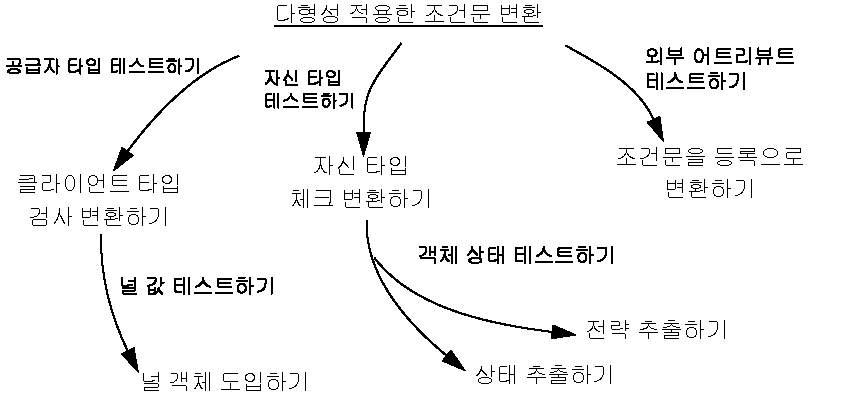
\includegraphics[width=\textwidth]{oldTransformMap.pdf}
\caption{조건부 변환을 다형성으로 구성하는 패턴 간의 관계}
\figlabel{TransformMap}
\end{center}
\end{figure}

\figref{TransformMap}은 패턴들 간의 관계와 차이점을 요약해서 보여준다.

\begin{bulletlist}
\item \patref{자신 타입 체크 변환하기}{TransformSelfTypeChecks}는 각 타입 케이스에 대해 \emph{서브클래스 도입}을 통해 프로바이더 클래스에서 타입 정보에 대한 조건부를 제거한다. 조건부 코드는 새 하위 클래스 중 하나의 인스턴스에 대한 단일 다형성 메서드 호출로 대체된다.

\item \patref{클라이언트 타입 검사 변환하기}{TransformClientTypeChecks}는 클라이언트 클래스의 타입 정보에 대한 조건부를 각 프로바이더 클래스에 \emph{새 메서드 도입}으로 변환합니다. 조건문은 새 메서드에 대한 단일 다형성 호출로 대체된다.

\item \patref{상태 추출하기}{FactorOutState}는 테스트 중인 타입 정보가 동적으로 변경될 수 있는 \patref{자신 타입 체크 변환하기}{TransformSelfTypeChecks}의 특수한 경우를 처리한다. \emph{변하는 상태를 모델링하기 위해 프로바이더 클래스에 \patref{상태}{State} 객체가 도입된다.} 그리고, 조건은 새 상태(State) 객체의 메서드 호출로 대체된다.

\item \patref{전략 추출하기}{FactorOutStrategy}는 \patref{자신 타입 체크 변환하기}{TransformSelfTypeChecks}의 또 다른 특수한 경우이다. 의 특수한 경우로, 다양한 프로바이더 사례를 처리하는 알고리즘이 \emph{새로운 \patref{전략}{Strategy} 객체 도입}에 의해 추출된다. \patref{상태 추출하기}{FactorOutState}와의 주요 차이점은 상태가 아닌 알고리즘이 동적으로 달라질 수 있다는 점이다.

\item \patref{널 객체 도입하기}{IntroduceNullObject}는 \patref{클라이언트 타입 검사 변환하기}{TransformClientTypeChecks}의 특수한 경우를 다룹니다. 이는 수행되는 테스트에서 프로바이더가 정의되어 있는지 여부를 확인한다. 조건은 적절한 기본 동작을 구현하는\emph{\patref{널 객체}{NullObject}}를 도입하여 제거한다.

\item \patref{조건문을 등록으로 변환하기}{TransformConditionalsIntoRegistration}은 처리할 객체의 일부 속성에 따라 조건문이 외부 도구를 시작하는 상황을 다룬다. 해결책은 도구가 플러그인으로 등록되는조회 서비스를 도입하는 것이다. 그런 다음 조건은 등록된 플러그인에 대한 간단한 조회로 대체된다. 그러면 도구 사용자를 변경하지 않고도 새 플러그인을 추가하거나 제거할 수 있으므로 솔루션은 완전히 동적이다. 
\end{bulletlist}

%=================================================================
%:PATTERN -- {Transform Self Type Checks}
\pattern{자신 타입 체크 변환하기}{TransformSelfTypeChecks}

\intent{서브클래스를 구현한 후크 메서드 호출로 복잡한 조건문을 대체하여 클래스의 확장성을 개선한다.}

\subsection*{문제}

클래스는 객체의 현재 '타입'을 나타내는 일부 속성을 테스트하는 복잡한 조건문에 여러 가지 가능한 동작을 묶어두기 때문에 수정하거나 확장하기가 어렵다.

\emph{이 문제는 다음과 같은 이유로 어렵다.}

\begin{bulletlist}
\item 개념적으로 간단한 확장이지만 조건부 코드에는 많은 변경이 필요하다.

\item 조건부 코드가 포함된 메서드를 복제하고 수정하지 않으면 서브클래싱이 거의 불가능하다.

\item 새 동작을 추가하면 항상 동일한 메서드 집합이 변경되고 항상 조건부 코드에 새 Case 문이 추가된다.
\end{bulletlist}

\emph{그러나 이 문제를 해결할 수 있는 이유는 다음과 같다.}

\begin{bulletlist}
\item 자체 타입 검사는 다형성을 시뮬레이션한다. 조건부 코드는 대신 어떤 서브클래스를 가져야 하는지 알려준다.
\end{bulletlist}

\subsection*{해결}

복잡한 조건 분기가 있는 메서드를 식별한다. 각각의 경우 조건부 코드를 새로운 훅 메서드 호출로 대체하자. 조건의 경우에 해당하는 서브클래스를 식별하거나 도입한다. 이러한 각 서브 클래스에서 원래 Case 문에서 해당 케이스에 해당하는 코드를 사용하여 후크 메서드를 구현한다.

\subsubsection*{탐지}

대부분의 경우 코드를 작업하는 동안 타입 구분이 눈에 띄기 때문에 굳이 어디에서 검사가 이루어지는지 감지할 필요가 없다. 그러나 시스템의 알려지지 않은 부분에 유사한 관행이 있는지 신속하게 평가할 수 있는 간단한 기술을 갖는 것은 흥미로울 수 있다. 이는 시스템 상태를 평가하는 데 유용한 정보 소스가 될 수 있다.

\begin{bulletlist}
\item 타입 정보를 모델링하는 객체의 일부 불변 속성에 대한 복잡한 결정 구조를 가진 긴 메서드를 찾는다. 특히 생성자에서 설정되고 변경되지 않는 속성을 찾아보자.

\item 유형 정보를 모델링하는 데 사용되는 속성은 일반적으로 일부 열거형 또는 일부 유한한 상수 값 집합에서 값을 가져온다. 이름이 일반적으로 클래스에 연결될 것으로 예상되는 엔티티 또는 개념을 나타내는 상수 정의(예: \lct{RetiredEmployee} 또는 \lct{PendingOrder})를 찾아보자. 조건문은 일반적으로 고정 속성의 값을 이러한 상수 값 중 하나와 비교하기만 한다.

\item 특히 \emph{여러} 메서드가 동일한 속성을 켜는 클래스를 찾아보세요. 이는 속성이 타입을 시뮬레이션하는 데 사용되고 있다는 또 다른 일반적인 신호이다.

\item Case 문이 포함된 메서드는 길이가 긴 경향이 있으므로 코드 줄별로 메서드를 정렬하거나 크기에 따라 클래스 및 메서드를 시각화하는 도구를 사용하는 것이 도움이 될 수 있다. 또는 조건문이 많은 클래스나 메서드를 검색할 수도 있다.

\item 클래스 구현을 별도의 파일에 저장하는 것이 일반적인 \ind{C++} 또는 \ind{Java}와 같은 언어의 경우 조건 키워드(\lct{if}, \lct{else}, \lct{case} 등)의 발생 빈도를 검색하고 세는 것이 간단하다. 예를 들어 \ind{UNIX} 시스템에서는 다음과 같이 할 수 있다.

\begin{code}
grep 'switch' `find . -name "*.cxx" -print`
\end{code}

이 명령은 디렉터리 트리에서 확장자가 \lct{.cxx}인 파일 중 \lct{switch}가 포함된 모든 파일을 열거한다. agrep와 같은 다른 텍스트 처리 도구는 더 세분화된 쿼리를 생성할 수 있는 가능성을 제공한다. ind{Perl}과 같은 텍스트 처리 언어는 일부 종류의 쿼리, 특히 여러 줄에 걸쳐 있는 쿼리를 평가하는 데 더 적합할 수 있다.

\item \emph{C/C++:}
레거시 C 코드는 union 타입을 사용하여 클래스를 시뮬레이션할 수 있다. 일반적으로 union 타입은 실제 타입을 인코딩하는 하나의 데이터 멤버를 갖는다. 이러한 데이터 멤버를 전환하는 조건문을 찾아 union을 캐스팅할 타입과 사용할 동작을 결정하자.

C++에서는 void 포인터로 선언된 데이터 멤버가 있는 클래스를 찾는 것이 매우 일반적이다. 다른 데이터 멤버의 값에 따라 이러한 포인터를 주어진 타입으로 형변환하는 조건문을 찾아보자. 타입 정보는 열거형 또는 (더 일반적으로) 상수 정수 값으로 인코딩할 수 있다.

\item \emph{\ind{Ada}:}
Ada 83은 다형성(또는 하위 프로그램 액세스 타입)을 지원하지 않았기 때문에, 다형성을 시뮬레이션하기 위해 구별된 레코드 타입(discreminated record type)을 사용하는 경우가 많다. 일반적으로 열거 타입은 여러 변형을 제공하며, 다형성으로의 변환은 Ada95에서는 간단하다.

\item \emph{\ind{Smalltalk}:}
Smalltalk는 타입을 조작하는 몇 가지 방법만 제공한다. 명시적 타입 검사를 나타내는 \lct{isMemberOf:}와 \lct{isKindOf:} 메서드의 응용 프로그램을 찾아보자. 타입 검사는 \lct{self class = anotherClass}와 같은 테스트 또는 계층 구조 전체에서 \lct{isSymbol}, \lct{isString}, \lct{isSequenceable}, \lct{isInteger}와 같은 메서드를 사용하여 속성 테스트를 통해 수행될 수도 있다.
\end{bulletlist}

\subsubsection*{단계}

\begin{figure}[tb]
\begin{center}
\includegraphics[width=\textwidth]{TransformTypeCheck}
\caption{명시적 타입 검사를 자체 다형성 메서드 호출로 변환}
\figlabel{TransformTypeCheck}
\end{center}
\end{figure}


\begin{enumerate}
\item 변환할 클래스와 그 클래스가 구현하는 다양한 개념적 클래스를 식별한다. 열거 타입이나 상수 집합이 이를 잘 문서화할 수 있다.

\item 구현되는 각 동작에 대해 새 하위 클래스를 도입한다(\figref{TransformTypeCheck} 참조). 클라이언트가 원래 클래스가 아닌 새 서브클래스를 인스턴스화하도록 수정한다. 테스트를 실행한다.

\item 조건문을 통해 다양한 동작을 구현하는 원래 클래스의 모든 메서드를 식별한다. 조건문이 다른 문으로 둘러싸여 있는 경우 별도의 보호된 후크 메서드로 이동시킨다. 각 조건문이 자체 메서드를 차지하면 테스트를 실행한다.

\item 조건문의 Case 문을 해당 하위 클래스로 반복적으로 이동하여 주기적으로 테스트를 실행한다.

\item 조건부 코드가 포함된 메서드는 이제 모두 비어 있어야 한다. 이를 추상 메서드로 대체하고 테스트를 실행하자.

\item 또는 적절한 기본 동작이 있는 경우 새 계층 구조의 루트에서 이를 구현하자.

\item 인스턴스화할 서브클래스를 결정하는 데 필요한 로직이 사소하지 않은 경우 이 로직을 새 계층 구조 루트의 팩토리 메서드로 캡슐화하는 것을 고려하자. 새 팩토리 메서드를 사용하도록 클라이언트를 업데이트하고 테스트를 실행한다.
\end{enumerate}

\subsection*{트레이드오프}

\subsubsection*{장점}

\begin{bulletlist}
\item 이제 모든 동작을 포함하는 단일 클래스의 메서드 집합을 변경하지 않고도 새로운 동작을 증분 방식으로 추가할 수 있다. 이제 특정 동작을 다른 변형과 독립적으로 이해할 수 있다. 

\item 새 동작은 다른 동작과 독립적으로 데이터를 나타내므로 가능한 간섭을 최소화하고 분리된 동작의 이해도를 높일 수 있다. 

\item 이제 모든 동작이 공통 인터페이스를 공유하므로 가독성이 향상된다.
\end{bulletlist}

\subsubsection*{단점}

\begin{bulletlist}
\item 이제 모든 동작이 여러 개의 관련 추상화로 분산되어 있으므로 동작에 대한 개요를 파악하기가 더 어려워질 수 있다. 그러나 개념이 서로 연관되어 있고 추상 클래스로 표현되는 인터페이스를 공유하므로 문제가 줄어든다. 

\item 클래스 수가 많으면 디자인이 더 복잡해지고 잠재적으로 이해하기 어려워진다. 원래 조건문이 단순하다면 이 변환을 수행할 가치가 없을 수도 있다.

\item 명시적 타입 검사가 항상 문제가 되는 것은 아니며 때로는 용인할 수 있다. 새 클래스를 만들면 애플리케이션의 추상화 수가 증가하고 네임스페이스가 복잡해질 수 있다. 따라서 다음과 같은 경우에는 명시적 타입 검사를 새 클래스 생성의 대안으로 사용할 수 있다.
	\begin{bulletlist}
	\item 메서드 선택이 고정되어 있고 향후에 진화하지 않을 집합이다. 그리고, 
	\item 몇 군데에서만 타입 검사가 수행된다.
	\end{bulletlist}
\end{bulletlist}

\subsubsection*{어려움}

\begin{figure}[tb]
\begin{center}
\includegraphics[width=\textwidth]{TransformDelegation}
\caption{클래스를 하위 클래스화할 수 없는 경우 단순 델리게이션과 \patref{자신 타입 체크 변환하기}{TransformSelfTypeChecks}를 결합}
\figlabel{TransformDelegation}
\end{center}
\end{figure}
%:HERE<==

\begin{bulletlist}
\item 필수 하위 클래스가 아직 존재하지 않기 때문에 여러 타입을 시뮬레이션하는 데 조건문이 사용되는 경우를 구분하기 어려울 수 있다.

\item 변환된 클래스의 인스턴스가 원래 생성되었다면 이제 다른 하위 클래스의 인스턴스를 생성해야 한다. 인스턴스화가 클라이언트 코드에서 발생한 경우 이제 해당 코드를 올바른 클래스를 인스턴스화하도록 조정해야 한다. 클라이언트에서 이러한 복잡성을 숨기려면 팩토리 객체 또는 메서드가 필요할 수 있다.

\item 클라이언트의 소스 코드에 액세스할 수 없는 경우 생성자에 대한 호출을 변경할 수 없으므로 이 패턴을 적용하기 어렵거나 불가능할 수 있다. 

\item Case 문이 둘 이상의 속성을 테스트하는 경우 더 복잡한 계층 구조를 지원해야 할 수 있으며, 여러 상속이 필요할 수도 있다. 클래스를 각각 고유한 계층 구조를 가진 부분으로 분할하는 것을 고려해 보자.

\item 원래 조건문을 포함하는 클래스를 서브클래싱할 수 없는 경우, \patref{자신 타입 체크 변환하기}{TransformSelfTypeChecks}를 델리게이션으로 구성할 수 있다. 원래 클래스의 상태와 동작의 일부를 메서드가 델리게이션할 별도의 클래스로 이동하여 다른 계층 구조에서 다형성을 활용하는 것이 \figref{TransformDelegation}에서 설명하는 아이디어이다.
\end{bulletlist}

\subsubsection*{레거시 솔루션이 최종 솔루션인 경우}

그럼에도 불구하고 명시적 타입 검사가 올바른 해결책이 될 수 있는 몇 가지 상황이 있다.

\begin{bulletlist}
\item 조건부 코드는 특수 도구에서 생성될 수 있다. 예를 들어 어휘 분석기와 구문 분석기는 우리가 피하고자 하는 종류의 조건문 코드를 포함하도록 자동으로 생성될 수 있다. 그러나 이러한 경우 생성된 클래스는 수동으로 확장하지 말고 수정된 사양에서 간단히 다시 생성해야 한다.
\end{bulletlist}

\subsection*{예시}

우리는 메시지를 전송하여 대규모의 물리적 기계를 제어하는 복잡한 시스템을 작업했다. 이러한 메시지는 \lct{Message} 클래스로 표현되며 다양한 타입이 있을 수 있다.

\begin{figure}[h]
\begin{center}
\includegraphics[width=0.9\textwidth]{TransformBefore}
\caption{초기 디자인 및 소스 코드}
\figlabel{TransformBefore}
\end{center}
\end{figure}

\subsubsection*{이전}

메시지 클래스는 코드와 그림에 표시된 것처럼 네트워크 연결을 통해 전송하기 위해 직렬화해야 하는 두 가지 종류의 메시지(\lct{TEXT} 및 \lct{ACTION})를 래핑한다. 새로운 종류의 메시지(예: \lct{VOICE})를 보낼 수 있기를 원하지만 이를 위해서는 \figref{TransformBefore}에 표시된 것처럼 \lct{Message}의 여러 메서드를 변경해야 한다. 

\begin{figure}[htb]
\begin{center}
\includegraphics[width=0.9\textwidth]{TransformAfter}
\caption{결과 계층 구조 및 소스 코드}
\figlabel{TransformAfter}
\end{center}
\end{figure}

\subsubsection*{이후}

\lct{Message}는 개념적으로 두 개의 다른 클래스인 \lct{Text\_Message}와 \lct{Action\_Message}를 구현하므로 \figref{TransformAfter}에 표시된 것처럼 이들을 \lct{Message}의 서브클래스로 도입된다. 새 클래스에 대한 생성자를 도입하고, 클라이언트가 \lct{Message}가 아닌 \lct{Text\_Message} 및 \lct{Action\_Message} 인스턴스를 생성하도록 수정하고, \lct{set\_value()} 메서드를 제거한다. 이 시점에서 회귀 테스트가 실행되어야 한다.

이제 \lct{type} 변수를 켜는 메서드를 찾는다. 각각의 경우, 스위치가 이미 전체 메서드를 차지하고 있지 않는 한, 전체 Case 문은 별도의 보호된 후크 메서드로 이동한다. \lct{send()}의 경우 이미 그렇게 되어 있으므로 후크 메서드를 도입할 필요가 없다. 다시 말하지만, 모든 테스트는 여전히 실행되어야 한다.

이제 \lct{Message}에서 그 서브클래스로 Case 문을 반복적으로 이동한다. \lct{Message::send()}의 \lct{TEXT} 케이스는 \lct{Text\_Message}::send()로 이동하고 \lct{ACTION} 케이스는 \lct{Action\_Message::send()}로 이동한다. 이러한 케이스를 이동할 때마다 테스트는 계속 실행되어야 한다.

마지막으로, 원래의 \lct{send()} 메서드는 이제 비어 있으므로 추상적으로 재선언할 수 있다(예: \lct{virtual void send(Channel) = 0}). 다시 테스트가 실행되어야 한다. 

\subsection*{근거}

여러 데이터 타입으로 가장한 클래스는 디자인을 이해하고 확장하기 어렵게 만든다. 명시적 타입 검사를 사용하면 여러 가지 동작을 혼합하는 긴 메서드가 생성된다. 새로운 동작을 도입하려면 새로운 동작을 나타내는 새로운 클래스 하나를 지정하는 대신 모든 메서드를 변경해야 한다.

이러한 클래스를 여러 데이터 타입을 명시적으로 나타내는 계층 구조로 변환하면 단일 데이터 타입과 관련된 모든 코드를 한데 모아 응집도를 높이고, 일정량의 중복 코드(즉, 조건부 테스트)를 제거하며, 디자인을 더 투명하게 만들어 결과적으로 유지보수성을 높일 수 있다.

\subsection*{관련 패턴}

\patref{자신 타입 체크 변환하기}{TransformSelfTypeChecks}에서 변환할 조건은 클래스 자체의 속성으로 표현되는 타입 정보를 테스트한다.

조건문이 호스트 객체의 \emph{변경가능한(mutable)} 상태를 테스트하는 경우, 대신 \patpgref{상태 추출하기}{FactorOutState} 또는 \patpgref{전략 추출하기}{FactorOutStrategy}를 적용하는 것을 고려하자.

조건이 프로바이더 클래스 자체가 아닌 \emph{클라이언트}에서 발생하는 경우 \patpgref{클라이언트 타입 검사 변환하기}{TransformClientTypeChecks}를 적용하는 것을 고려하자.

조건문 코드가 \emph{세 번째 핸들러 객체 선택하기}를 위해 두 번째 객체의 일부 타입 속성을 테스트하는 경우 대신 \patpgref{조건문을 등록으로 변환하기}{TransformConditionalsIntoRegistration}을 적용하는 것을 고려하자. 

%=================================================================
%:PATTERN -- {Transform Client Type Checks}
\pattern{클라이언트 타입 검사 변환하기}{TransformClientTypeChecks}

\intent{프로바이더의 타입을 검사하는 조건문 코드를 새 프로바이더 메서드에 대한 다형성 호출로 변환하여 클라이언트/프로바이더 결합도를 줄인다.}

\subsection*{문제}

클라이언트가 명시적으로 프로바이더의 타입을 확인하고 프로바이더 코드를 작성할 책임이 있는 경우, 클라이언트와 서비스 프로바이더 간의 결합도를 어떻게 줄일 수 있는가?

\emph{이 문제는 다음과 같은 이유로 어렵다.}

\begin{bulletlist}
\item 프로바이더 계층 구조에 새 하위 클래스를 추가하려면 특히 테스트가 많이 필요한 클라이언트 변경을 해야 한다.

\item 클라이언트가 프로바이더의 책임이어야 하는 작업을 수행하기 때문에 클라이언트와 프로바이더는 결합도가 높은 경향이 있다. 
\end{bulletlist}

\emph{그러나 이 문제를 해결할 수 있는 이유는 다음과 같다.}

\begin{bulletlist}
\item 조건문은 동작을 옮겨두어야 하는 클래스를 알려준다.
\end{bulletlist}

\subsection*{해결}

프로바이더 계층 구조에 새 메서드를 도입한다. 클라이언트 조건의 해당 케이스를 해당 클래스로 이동하여 프로바이더 계층 구조의 각 하위 클래스에서 새 메서드를 구현한다. 클라이언트의 전체 조건문을 새 메서드에 대한 간단한 호출로 대체한다.

\subsubsection*{탐지}

\patref{자신 타입 체크 변환하기}{TransformSelfTypeChecks}에서 설명한 것과 기본적으로 동일한 기술을 적용하여 Case 문을 감지하되, 계층 구조를 구현하는 별도의 서비스 프로바이더의 타입을 테스트하는 조건을 찾는다. 또한 동일한 프로바이더 계층 구조의 다른 클라이언트에서 발생하는 Case 문도 찾아야 한다.

\begin{bulletlist}
\item \emph{\ind{C++}:}
레거시 C++ 코드는 런타임 타입 정보(\ind{RTTI})를 사용하지 않을 가능성이 높다. 대신, 타입 정보는 현재 클래스를 나타내는 열거형에서 값을 가져오는 데이터 멤버에 인코딩될 가능성이 높다. 이러한 데이터 멤버를 전환하는 클라이언트 코드를 찾아보자.

\item \emph{\ind{Ada}:}
타입 테스트 감지는 두 가지 경우에 해당한다. 계층 구조가 단일 판별 레코드로 구현된 경우 판별자에 대한 Case 문장을 찾을 수 있다. 계층 구조가 태그가 지정된 타입으로 구현된 경우 타입에 대한 Case 문을 작성할 수 없으며(불연속적이지 않음), 대신 if-then-else 구조가 사용된다.

\item \emph{\ind{Smalltalk}:}
\patref{자신 타입 체크 변환하기}{TransformSelfTypeChecks}에서와 같이 \lct{isMemberOf:} 및 \lct{isKindOf:}의 적용과 \lct{self class = anotherClass} 같은 테스트를 찾는다.

\item \emph{\ind{Java}:}
특정 알려진 클래스에서 객체의 멤버십을 테스트하는 연산자 \lct{instanceof}의 응용 프로그램을 찾아보자. Java의 클래스는 Smalltalk에서처럼 객체가 아니지만, 가상 머신에 로드되는 각 클래스는 \lct{java.lang.Class}의 단일 인스턴스로 표현된다. 따라서 테스트를 수행하여 두 개의 객체 \lct{x}와 \lct{y}가 같은 클래스에 속하는지 확인할 수 있다.
\begin{code}
x.getClass() == y.getClass()
\end{code}
또는 클래스 이름을 비교하여 클래스 멤버십을 테스트할 수도 있다.
\begin{code}
x.getClass().getName().equals(y.getClass().getName())
\end{code}

\end{bulletlist}

\begin{figure}[tb]
\begin{center}
\includegraphics[width=\textwidth]{TransformClient}
\caption{다형성 메서드 호출로 호출해야 하는 클라이언트의 메서드를 결정하는 데 사용되는 명시적 타입 검사 변환이다.}
\figlabel{TransformClient}
\end{center}
\end{figure}

\subsubsection*{단계}

\begin{enumerate}
\item 명시적 타입 검사를 수행하는 클라이언트를 식별한다.

\item 조건문 코드에서 수행되는 작업을 나타내는 프로바이더 계층 구조의 루트에 빈 메서드를 새로 추가한다(\figref{TransformClient} 참조).

\item 조건문의 Case 문을 일부 프로바이더 클래스로 반복적으로 이동하여 해당 메서드 호출로 대체한다. 각 이동 후에는 회귀 테스트를 실행해야 한다.

\item 모든 메서드가 이동되면 조건문의 각 Case 문이 새 메서드 호출로 구성되므로 전체 조건문을 새 메서드 호출 한 번으로 대체할 수 있다.

\item 프로바이더의 루트에서 메서드를 추상화하는 것을 고려하자. 또는 여기에 적절한 기본 동작을 구현하자.
\end{enumerate}

\subsubsection*{고려할 다른 단계}

\begin{bulletlist}
\item 여러 클라이언트가 정확히 동일한 테스트를 수행하고 동일한 동작을 수행하는 경우가 있을 수 있다. 이 경우 클라이언트 중 하나를 변환한 후 중복된 코드를 단일 메서드 호출로 대체할 수 있다. 클라이언트가 다른 테스트를 수행하거나 다른 조치를 취하는 경우 각 조건에 대해 패턴을 한 번씩 적용해야 한다.

\item Case 문이 프로바이더 계층 구조의 모든 구체적인 클래스를 포함하지 않는 경우, 관련 클래스의 공통 수퍼클래스로 새로운 추상 클래스를 도입해야 할 수 있다. 그러면 새 메서드는 관련 하위 트리에만 도입된다. 또는 기존 상속 계층 구조에서 이러한 추상 클래스를 도입할 수 없는 경우 루트에서 비어 있는 기본 구현 또는 부적절한 클래스를 호출될 경우 예외를 발생시키는 구현을 사용하여 메서드를 구현하는 것을 고려하자.

\item 조건문이 중첩된 경우 패턴을 재귀적으로 적용해야 할 수 있다.
\end{bulletlist}

\subsection*{트레이드오프}

\subsubsection*{장점}

\begin{bulletlist}
\item 프로바이더 계층은 다른 클라이언트도 사용할 수 있는 새로운 다형성 서비스를 제공한다.

\item 이제 클라이언트의 코드가 더 잘 정리되어 더 이상 프로바이더가 책임져야 하는 문제를 처리할 필요가 없다.

\item 단일 프로바이더의 동작에 관한 모든 코드가 이제 한 곳에 모인다.

\item 프로바이더 계층 구조가 통일된 인터페이스를 제공하므로 클라이언트에 영향을 주지 않고 프로바이더를 수정할 수 있다. 
\end{bulletlist}

\subsubsection*{단점}

\begin{bulletlist}
\item 때로는 다양한 케이스를 처리하는 코드를 한 곳에서 보는 것이 편리할 때가 있다. \patref{클라이언트 타입 검사 변환하기}{TransformClientTypeChecks}는 로직을 개별 프로바이더 클래스에 재배포하므로 전체적으로 살필 수 있는 기회는 손실된다.
\end{bulletlist}

\subsubsection*{어려움}

\begin{bulletlist}
\item 일반적으로 프로바이더 클래스의 인스턴스는 이미 생성되어 있으므로 인스턴스 생성을 찾을 필요가 없지만 인터페이스를 리팩터링하면 프로바이더 클래스의 모든 클라이언트에 영향을 미치므로 이러한 작업의 전체 결과를 고려하지 않고 수행해서는 안 된다.
\end{bulletlist}

\subsubsection*{레거시 솔루션이 최종 솔루션인 경우}

그럼에도 불구하고 클라이언트 타입 검사는 프로바이더 인스턴스가 아직 존재하지 않거나 해당 클래스를 확장할 수 없는 경우 올바른 솔루션이 될 수 있다.

\begin{bulletlist}
\item 인스턴스화할 클래스를 알기 위해 타입 변수를 테스트해야 하는 \patpgref{추상 팩토리}{AbstractFactory} 객체가 있을 수 있다. 예를 들어 팩토리는 텍스트 파일 표현에서 객체를 스트리밍하고 스트리밍된 객체가 어느 클래스에 속해야 하는지 알려주는 일부 변수를 테스트할 수 있다.

\item 레거시 GUI 라이브러리와 같이 객체 지향이 아닌 라이브러리와 인터페이스하는 소프트웨어는 개발자가 디스패치를 수동으로 시뮬레이션해야 할 수 있다. 이러한 경우 프로시저 라이브러리에 대한 객체 지향 파사드를 개발하는 것이 비용 효율적인지 의문이다.

\item 프로바이더 계층 구조가 고정된 경우(예: 소스 코드를 사용할 수 없기 때문에) 동작을 프로바이더 클래스로 전송할 수 없다. 이 경우 래퍼 클래스를 정의하여 프로바이더 클래스의 동작을 확장할 수 있지만 래퍼 정의의 복잡성이 추가되어 이점을 없을 수 있다.
\end{bulletlist}

\subsection*{예시}

\subsubsection*{예전}

다음 \ind{C++} 코드는 클라이언트가 수행할 작업을 결정하기 위해 명시적으로 전화의 검사 인스턴스를 타입으로 지정해야 하므로 잘못 배치된 책임을 보여준다. 굵게 표시된 코드는 이 접근 방식의 어려움을 강조한다.

%:>>>HERE<<<

\begin{code}
class Telephone {
public:
	enum PhoneType {
		POTSPHONE, ISDNPHONE, OPERATORPHONE
		};
	Telephone() {}
	PhoneType phoneType() { return myType; }

private:
	PhoneType myType;
protected: 
	void setPhoneType(PhoneType newType) { myType = newType; }
};

class POTSPhone : public Telephone {

public: 
	POTSPhone() { setPhoneType(POTSPHONE); }
	void tourneManivelle();
	void call();
};
...

class ISDNPhone: public Telephone {
public:
	ISDNPhone() { setPhoneType(ISDNPHONE);}
	void initializeLine();
	void connect();
};
...

class OperatorPhone: public Telephone {
public: 
	OperatorPhone() { setPhoneType(OPERATORPHONE); }
	void operatorMode(bool onOffToggle);
	void call();
};

void initiateCalls(Telephone ** phoneArray, int numOfCalls) {
	for(int i = 0; i<numOfCalls ;i++ ) {
		Telephone * p = phoneArray[i];

		switch(p->phoneType()) {
		case Telephone::POTSPHONE: {
			POTSPhone *potsp = (POTSPhone *) p;
			potsp->tourneManivelle();
			potsp->call();
			break;
		}
		case Telephone::ISDNPHONE: {
			ISDNPhone *isdnp = (ISDNPhone *) p;
			isdnp->initializeLine();
			isdnp->connect();
			break;
		}
		case Telephone::OPERATORPHONE: {
			OperatorPhone *opp = (OperatorPhone *) p;
			opp->operatorMode(true);
			opp->call();
			break;
		}
		default:	cerr << "Unrecognized Phonetype" << endl;
		};
	}
}
\end{code}

\begin{figure}
\begin{center}
\includegraphics[width=\textwidth]{TransformPhone}
\caption{명시적 타입 검사를 다형성 메서드 호출로 변환한다.}
\figlabel{TransformPhone}
\end{center}
\end{figure}

\subsubsection*{이후}

패턴을 적용한 후 클라이언트 코드는 다음과 같이 표시된다.
(\figref{TransformPhone}도 참조하자.)
% In bold we highlight the changes:

\begin{code}
class Telephone {
public:
	Telephone() {}
	virtual void makeCall() = 0;
};

Class POTSPhone : public Telephone {
	void tourneManivelle();
	void call();
public: 
	POTSPhone() {}
	void makeCall();
};
void POTSPhone::makeCall() {
	this->tourneManivelle();
	this->call();
}

class ISDNPhone: public Telephone {
	void initializeLine();
	void connect();

public:
	ISDNPhone() { }
	void makeCall();
};
void ISDNPhone::makeCall() {
	this->initializeLine();
	this->connect();
}

class OperatorPhone: public Telephone {
	void operatorMode(bool onOffToggle);
	void call();
public: 
	OperatorPhone() { }
	void makeCall();
};
void OperatorPhone::makeCall() {
	this->operatorMode(true);
	this->call();
}
void initiateCalls(Telephone ** phoneArray, int numOfCalls) {
	for(int i = 0; i<numOfCalls ;i++ ) {
		phoneArray[i]->makeCall();
	}
}
\end{code}

\subsection*{근거}

리엘은 ``객체 타입에 대한 명시적 Case 문을 이용한 분석은 일반적으로 에러 상황이다. 대부분의 경우 다형성을 사용해야 한다.''고 했다 \cite{Riel96a}. 실제로 클라이언트의 명시적 타입 검사는 클라이언트와 프로바이더 간의 결합도를 높이기 때문에 책임이 잘못 배치되었다는 신호이다. 이러한 책임을 프로바이더에게 전가하면 다음과 같은 결과가 발생한다.

\begin{bulletlist}
\item 클라이언트는 모든 구체적인 하위 클래스 대신 프로바이더 계층의 루트만 명시적으로 알면 되므로 클라이언트와 프로바이더의 결합도가 더 약해진다.

\item 프로바이더 계층 구조는 클라이언트 코드를 손상시킬 가능성을 줄이면서 더 우아하게 진화할 수 있다.

\item 클라이언트 코드의 크기와 복잡성이 줄어든다. 클라이언트와 프로바이더 간의 협업이 더욱 추상화된다.

\item 기존 디자인에 암시되어 있던 추상화(예: 조건문의 Case 문 동작)가 메서드로 명시되어 다른 클라이언트에서 사용할 수 있다.

\item (동일한 조건문이 여러 번 발생하는 경우) 코드 중복이 줄어들 수 있다.
\end{bulletlist}

\subsection*{관련 패턴}

\patref{클라이언트 타입 검사 변환하기}{TransformClientTypeChecks}에서는 프로바이더 클래스의 타입 정보에 따라 조건이 만들어진다. \patref{널 객체 도입하기}{IntroduceNullObject}에서도 같은 상황이 발생하는데, 메서드를 호출하기 전에 널(Null) 값에 대한 조건문 테스트가 이루어진다. 이러한 관점에서 볼 때 \patref{널 객체 도입하기}{IntroduceNullObject}는 \patref{클라이언트 타입 검사 변환하기}{TransformClientTypeChecks}의 특수화(specialization)라고 할 수 있다. 

\patref{조건문을 등록으로 변환하기}{TransformConditionalsIntoRegistration}은 클라이언트의 조건이 인자를 처리할 제3의 객체(일반적으로 외부 애플리케이션 또는 도구)를 선택하는 데 사용되는 특수한 경우를 처리한다.

이 리엔지니어링 패턴의 핵심 리팩터링은 \patpgref{조건문을 다형성으로 치환하기}{ReplaceConditionalWithPolymorphism}으로 \cite{Fowl99a}에 설명된 단계를 참조할 수 있다.

%=================================================================
%:PATTERN -- {Factor out State}
\pattern{상태 추출하기}{FactorOutState}

\intent{개체의 상태에 대한 복잡한 조건문 코드를 \patref{상태}{State} 디자인 패턴을 적용하여 제거한다.}

\subsection*{문제}

현재 상태의 복잡한 평가에 따라 동작이 달라지는 클래스를 어떻게 더 확장 가능하게 만들 수 있을까?

\emph{이 문제는 다음과 같은 이유로 어렵다.}

\begin{bulletlist}
\item 객체의 메서드에 여러 개의 복잡한 조건문이 분산되어 있다. 새로운 동작을 추가하면 이러한 조건문에 미묘한 방식으로 영향을 미칠 수 있다.

\item 새로운 가능한 상태가 도입될 때마다 상태를 테스트하는 모든 메서드를 수정해야 한다.
\end{bulletlist}

\emph{그러나 이 문제를 해결할 수 있는 이유는 다음과 같다.}

\begin{bulletlist}
\item 객체의 인스턴스 변수는 일반적으로 각기 다른 추상 상태를 모델링하는 데 사용되며, 각 상태에는 고유한 동작이 있다. 이러한 추상 상태를 식별할 수 있다면 상태와 동작을 더 간단한 관련 클래스 집합으로 분해할 수 있다.
\end{bulletlist}

\subsection*{해결}

즉, 상태 종속 동작(state-dependent behavior)을 별도의 객체로 캡슐화하고, 이러한 객체에 대한 호출을 델리게이션하고, 이러한 상태 객체의 올바른 인스턴스를 참조하여 객체의 상태를 일관되게 유지하는 \patpgref{상태}{State} 패턴을 적용한다. (\figref{TransformState} 참조)

\patref{자신 타입 체크 변환하기}{TransformSelfTypeChecks}에서와 같이 정량화된 상태를 테스트하는 복잡한 조건부 코드를 상태 클래스에 대한 델리게이션 호출로 변환한다. \patpgref{상태}{State} 패턴을 적용하여 각 조건 사례를 별도의 상태 객체에 델리게이션한다. 이 문제에 대한 자세한 설명과 토론은 \patref{상태}{State}와 \patlangpgref{상태 패턴}{StatePatterns}를 읽어보기 바란다. \cite{Alpe98a} \cite{Dyso97a}. 여기서는 패턴의 리엔지니어링 측면에만 초점을 맞춘다.

\begin{figure}
\begin{center}
\includegraphics[width=0.8\textwidth]{TransformState}
\caption{명시적 상태 조건문를 사용하여 상태 패턴을 흉내 낸 것에서 상태 패턴이 적용된 상황으로 변환한다.}
\figlabel{TransformState}
\end{center}
\end{figure}

\subsubsection*{단계}

\begin{enumerate}
\item 상태의 인터페이스와 상태의 개수를 식별한다.

운이 좋으면 각 조건이 같은 방식으로 상태 공간을 분할하고 상태 수는 각 조건의 Case 문의 수와 같을 것이다. 조건이 겹치는 경우에는 더 세밀한 분할이 필요하다.

상태의 인터페이스는 상태 정보에 액세스하고 업데이트하는 방법에 따라 달라지며, 후속 단계에서 개선해야 할 수도 있다.

\item 상태의 인터페이스를 나타내는 새 추상 클래스 \lct{State}를 만든다.

\item 각 상태에 대해 \lct{State}의 새 클래스 서브클래스를 만든다.

\item 각 상태 클래스에서 1단계에서 식별한 인터페이스의 메서드를 새 메서드에 조건의 해당 코드를 복사하여 정의한다. \lct{Context}에서 인스턴스 변수의 상태가 \lct{State} 클래스의 올바른 인스턴스를 참조하도록 변경하는 것을 잊지 말자. \lct{State} 메서드는 항상 다음 상태 인스턴스를 참조하도록 \lct{Context}를 변경해야 할 책임이 있다. 

\item \lct{Context} 클래스에 새 인스턴스 변수를 추가한다.

\item \lct{State} 클래스에서 상태 전환을 호출하려면 \lct{State}에서 \lct{Context} 클래스로의 참조가 필요할 수 있다.

\item 기본 상태 클래스 인스턴스를 참조하도록 새로 생성된 인스턴스를 초기화한다.

\item 인스턴스 변수에 대한 호출을 델리게이션하도록 테스트가 포함된 \lct{Context} 클래스의 메서드를 변경한다.
\end{enumerate}

단계 4는 리팩터링 브라우저의 \patref{메서드 추출하기}{ExtractMethod} 작업을 사용하여 수행할 수 있다. 각 단계가 끝난 후에도 회귀 테스트는 계속 실행되어야 한다는 점에 유의하자. 중요한 단계는 동작이 새로운 상태 객체에 델리게이션되는 마지막 단계이다.

\subsection*{트레이드오프}

\subsubsection*{장점}

\begin{bulletlist}
\item \emph{제한적 영향:} 원래 클래스의 퍼블릭 인터페이스는 변경할 필요가 없다. 상태 인스턴스는 원래 객체에서 델리게이션을 통해 액세스되므로 클라이언트는 영향을 받지 않는다. 간단한 경우 이 패턴을 적용해도 클라이언트에 미치는 영향은 제한적이다.
\end{bulletlist}

\subsubsection*{단점}

\begin{bulletlist}
	\item 이 패턴을 체계적으로 적용하면 클래스 수가 폭발적으로 증가할 수 있다.

	\item 이 패턴은 다음과 같은 경우에 적용해서는 안 된다.

	\begin{bulletlist}
	\item 가능한 상태가 너무 많거나 상태 수가 고정되어 있지 않은 경우
	\item 코드에서 상태 전환이 언제 어떻게 발생하는지 파악하기 어려운 경우
	\end{bulletlist}
\end{bulletlist}

\subsubsection*{레거시 솔루션이 최종 솔루션인 경우}

이 패턴은 가볍게 적용해서는 안 된다.

\begin{bulletlist}
\item 상태가 명확하게 식별되고 변경되지 않을 것으로 알려진 경우 레거시 솔루션은 모든 상태 동작을 여러 하위 클래스에 분산하는 대신 기능별로 그룹화할 수 있는 이점이 있다.

\item 파서와 같은 특정 도메인에서는 상태에 대한 조건부로 인코딩된 테이블 기반 동작이 잘 이해되며, 상태 객체를 제외하면 코드를 이해하기 어렵고 따라서 유지보수성이 떨어질 수 있다.
\end{bulletlist}

\subsection*{알려진 용도}

\emph{Design Patterns Smalltalk Companion} \cite{Alpe98a}는 단계별 코드 변환에 대해 설명한다.

%=================================================================
%:PATTERN -- {Factor out Strategy}
\pattern{전략 추출하기}{FactorOutStrategy}
  
\intent{\patref{전략}{Strategy} 디자인 패턴을 적용하여 적합한 알고리즘을 선택하는 조건문 코드를 제거한다.}

\subsection*{문제}

어떤 변수 값의 테스트에 따라 동작이 달라지는 클래스를 어떻게 하면 더 확장 가능하게 만들 수 있을까?

\emph{이 문제는 다음과 같은 이유로 어렵다.}

\begin{bulletlist}
\item 조건문 코드가 포함된 모든 메서드를 수정하지 않고는 새로운 기능을 추가할 수 없다. 

\item 조건문 코드는 적용할 알고리즘에 대해 유사한 결정을 내리는 여러 클래스에 분산되어 있을 수 있다.
\end{bulletlist}

\emph{그러나 이 문제를 해결할 수 있는 이유는 다음과 같다.}

\begin{bulletlist}
\item 대체 동작은 본질적으로 상호 교환이 가능한다.
\end{bulletlist}

\subsection*{해결}

즉, 알고리즘 종속 동작을 다형성 인터페이스가 있는 별도의 객체로 캡슐화하고 이러한 객체에 대한 호출을 델리게이션하는 \patref{전략}{Strategy} 패턴을 적용한다(\figref{TransformStrategy} 참조). 

\begin{figure}[h]
\begin{center}
\includegraphics[width=\textwidth]{TransformStrategy}
\caption{명시적 전략 조건문으로 전략 패턴을 흉내낸 것에서 전략 패턴이 적용된 상황으로 변환한다.}
\figlabel{TransformStrategy}
\end{center}
\end{figure}

\subsubsection*{단계}
\begin{enumerate}
\item 전략 클래스의 인터페이스를 식별한다.

\item 전략의 인터페이스를 나타내는 새 추상 클래스 \lct{Strategy}를 만든다.

\item 식별된 각 알고리즘에 대해 \lct{Strategy}의 새 클래스 서브클래스를 만든다.

\item 테스트의 해당 코드를 메서드에 복사하여 각 전략 클래스에서 1단계에서 식별한 인터페이스의 메서드를 정의한다. 

\item 현재 전략을 참조하기 위해 \lct{Context} 클래스에 새 인스턴스 변수를 추가한다.

\item \lct{Context}가 유지 관리하는 정보에 대한 액세스를 제공하려면 \lct{Strategy}에서 \lct{Context} 클래스로의 참조가 필요할 수 있다(어려움 참조).

\item 기본 전략 인스턴스를 참조하도록 새로 생성된 인스턴스를 초기화한다.

\item 테스트를 제거하고 인스턴스 변수에 대한 호출을 델리게이션하여 테스트가 포함된 \lct{Context} 클래스의 메서드를 변경한다.
\end{enumerate}

단계 4는 리팩터링 브라우저의 \patref{메서드 추출하기}{ExtractMethod} 작업을 사용하여 수행할 수 있다. 각 단계가 끝난 후에도 회귀 테스트는 계속 실행되어야 한다는 점에 유의하자. 중요한 단계는 동작이 새로운 \lct{Strategy} 객체에 델리게이션되는 마지막 단계이다.

\subsection*{트레이드오프}

\subsubsection*{장점}

\begin{bulletlist}
\item \emph{제한적 영향:} 원래 클래스의 퍼블릭 인터페이스는 변경할 필요가 없다. \lct{Strategy} 인스턴스는 원래 객체에서 델리게이션을 통해 액세스되므로 클라이언트는 영향을 받지 않는다. 간단한 경우 이 패턴을 적용해도 클라이언트에 미치는 영향은 제한적이다. 그러나 이전에 구현된 모든 알고리즘이 이제 \lct{Strategy} 클래스로 이동하기 때문에 \lct{Context} 인터페이스가 축소된다. 따라서 이러한 메서드의 호출을 확인하고 케이스별로 결정해야 한다. 

\item 이 패턴을 적용하면 \lct{Context}의 인터페이스 수정에 영향을 주지 않고 새 전략을 플러그할 수 있다. 새 전략을 추가해도 \lct{Context} 클래스와 해당 클라이언트를 다시 컴파일할 필요가 없다. 

\item 이 패턴을 적용하면 \lct{Context} 클래스와 \lct{Strategy} 클래스의 인터페이스가 더 명확해진다.
\end{bulletlist}

\subsubsection*{단점}

\begin{bulletlist}
\item 이 패턴을 체계적으로 적용하면 클래스가 폭발적으로 늘어날 수 있다. 20개의 서로 다른 알고리즘이 있는 경우 각각 하나의 메서드만 있는 20개의 새 클래스를 갖고 싶지 않을 수 있다. 

\item 객체 폭발(Object explosion). 전략은 애플리케이션의 인스턴스 수를 증가시킨다.
\end{bulletlist}

\subsubsection*{어려움}

\begin{bulletlist}
\item \lct{Context}와 \lct{Strategy} 객체 간에 정보를 공유하는 방법에는 여러 가지가 있으며, 트레이드오프는 미묘할 수 있다. \lct{Strategy} 메서드가 호출될 때 정보를 인자로 전달하거나, \lct{Context} 객체 자체를 인자로 전달하거나, \lct{Strategy} 객체가 해당 컨텍스트에 대한 참조를 보유할 수 있다. \lct{Context}와 \lct{Strategy} 사이의 관계가 매우 동적인 경우 이 정보를 메서드 인자로 전달하는 것이 더 바람직할 수 있다. 이 문제에 대한 자세한 논의는 \patpgref{전략}{Strategy} 패턴에 대한 문헌에서 확인할 수 있다\cite{Gamm95a} \cite{Alpe98a}. 
\end{bulletlist}

\subsection*{예시}

\emph{Design Patterns Smalltalk Companion} \cite{Alpe98a}는 단계별 코드 변환에 대해 자세히 다룬다.

\subsection*{관련 패턴}

\patref{전략 추출하기}{FactorOutStrategy}의 증상과 구조는 \patref{상태 추출하기}{FactorOutState}와 비교해 볼 수 있다. 주요 차이점은 \patref{상태 추출하기}{FactorOutState}는 객체의 가능한 상태가 다른 동작을 식별하는 반면, \patref{전략 추출하기}{FactorOutStrategy}는 객체 상태와 무관한 상호 교환 가능한 알고리즘과 관련이 있다는 사실에 있다. \patref{전략 추출하기}{FactorOutStrategy}를 사용하면 기존 전략 개체에 영향을 주지 않고 새 전략을 추가할 수 있다.

%=================================================================
%:PATTERN -- {Introduce Null Object}
\pattern{널 객체 도입하기}{IntroduceNullObject}


\intent{\patref{널 객체}{NullObject} 디자인 패턴을 적용하여 null 값을 테스트하는 조건문 코드를 제거한다.}

\subsection*{문제}

널(null) 값에 대한 반복 테스트가 있는 경우 클래스의 수정 및 확장을 쉽게 하려면 어떻게 해야 할까?

\emph{이 문제는 다음과 같은 이유로 어렵다.}

\begin{bulletlist}
\item 클라이언트 메서드는 실제로 메서드를 호출하기 전에 항상 특정 값이 널(null)이 아닌지 테스트한다.

\item 클라이언트 계층 구조에 새 하위 클래스를 추가하려면 일부 프로바이더 메서드를 호출하기 전에 널(null) 값을 테스트해야 한다.
\end{bulletlist}

\emph{그러나 이 문제를 해결할 수 있는 이유는 다음과 같다.}

\begin{bulletlist}
\item 클라이언트는 프로바이더가 널(null) 값을 나타내는지 알 필요가 없다.
\end{bulletlist}

\subsection*{해결}

즉, 클라이언트 클래스가 널 테스트를 수행할 필요가 없도록 널 동작을 별도의 프로바이더 클래스로 캡슐화하여 \patpgref{널 객체}{NullObject} 패턴을 적용한다.

\subsubsection*{탐지}

관용적인 널 테스트를 찾아보자. 

널 테스트는 프로그래밍 언어와 테스트 대상 엔티티의 종류에 따라 다른 형태를 취할 수 있다. 예를 들어 \ind{Java}에서 널 객체 참조의 값은 \lct{null}인 반면, \ind{C++}에서 널 객체 포인터의 값은 0이다.

\subsubsection*{단계}

\index{파울러, 마틴}
파울러는 필요한 리팩터링 단계에 대해 자세히 설명한다 \cite{Fowl99a}.
\begin{enumerate}
\item 널 동작에 필요한 인터페이스를 식별한다. (일반적으로 널이 아닌 객체의 인터페이스와 동일하다.)

\item \lct{RealObject} 클래스의 수퍼클래스로서 새 추상 수퍼클래스를 만든다.

\item 이름이 \lct{No} 또는 \lct{Null}로 시작하는 추상 슈퍼클래스의 새 하위 클래스를 만든다.

\item Null Object 클래스에 기본 메서드를 정의한다.

\item 검사한 인스턴스 변수 또는 구조체를 초기화하여 이제 Null Object 클래스의 인스턴스를 하나 이상 보유하도록 한다.

\item 클라이언트에서 조건부 테스트를 제거한다.
\end{enumerate}

여전히 깔끔한 방식으로 null 값을 테스트하고 싶다면 파울러\cite{Fowl99a}가 설명한 대로 \lct{RealObject} 및 Null Object 클래스에 \lct{isNull}이라는 쿼리 메서드를 도입할 수 있다.

\begin{figure}
\begin{center}
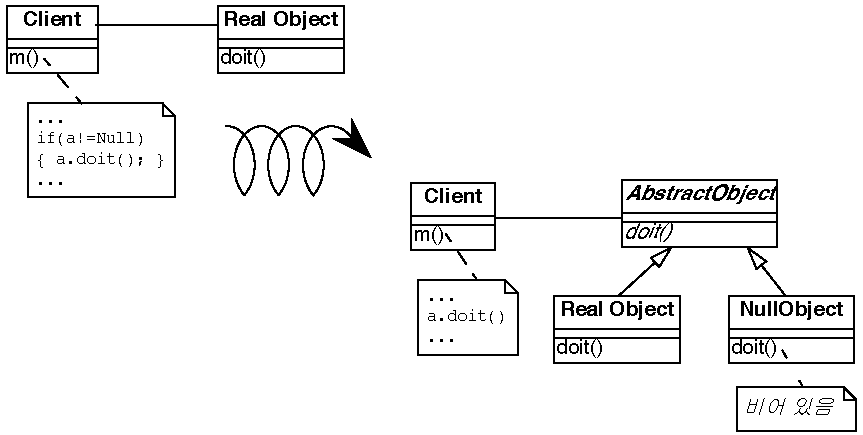
\includegraphics[width=\textwidth]{oldTransformNullObject.pdf}
\caption{명시적인 널 값 테스트에 기반한 상황에서 널 객체가 도입된 상황으로 변환한다.}
\figlabel{TransformNullObject}
\end{center}
\end{figure}

\subsection*{트레이드오프}

\subsubsection*{장점}

\begin{bulletlist}
\item 패턴을 적용한 후 클라이언트 코드가 훨씬 간단해졌다.

\item 프로바이더의 인터페이스를 수정할 필요가 없으므로 패턴을 적용하기가 비교적 간단하다.
\end{bulletlist}

\subsubsection*{단점}

\begin{bulletlist}
\item 프로바이더 계층 구조가 더 복잡해진다.
\end{bulletlist}

\subsubsection*{어려움}

\begin{bulletlist}
	\item 여러 클라이언트가 널(Null) 객체의 합리적인 기본 동작에 동의하지 않을 수 있다. 이 경우 여러 개의 널(Null) 객체 클래스를 정의해야 할 수 있다.
\end{bulletlist}

\subsubsection*{레거시 솔루션이 최종 솔루션인 경우}

\begin{bulletlist}
\item 클라이언트가 공통 인터페이스에 동의하지 않는 경우.

\item 변수를 직접 사용하는 코드가 거의 없거나 변수를 사용하는 코드가 한 곳에 잘 캡슐화되어 있는 경우.
\end{bulletlist}

\subsection*{예시}

\index{울프, 바비}
다음 \ind{Smalltalk} 코드는 울프\cite{Wool98a}의 저작에서 가져온 것이다. 처음에 이 코드에는 다음과 같은 명시적 널(null) 테스트가 포함되어 있다.

\begin{code}
VisualPart>>objectWantedControl
	...
	^ctrl isNil 
		ifFalse:
			[ctrl isControlWanted
				ifTrue:[self]
				ifFalse:[nil]]
\end{code}

이코드는 다음과 같이 변환가능하다.

\begin{code}
VisualPart>>objectWantedControl
	...
	^ctrl isControlWanted
				ifTrue:[self]
				ifFalse:[nil]
Controller>>isControlWanted
	^self viewHasCursor
NoController>>isControlWanted
	^false
\end{code}


%=================================================================
%:PATTERN -- {Transform Conditionals into Registration}
\pattern{조건문을 등록으로 변환하기}{TransformConditionalsIntoRegistration}


\intent{클라이언트의 조건문을 등록(registration) 메커니즘으로 대체하여 시스템의 모듈성을 개선한다.}

\subsection*{문제}

도구를 추가하거나 제거해도 클라이언트의 코드가 변경되지 않도록 서비스를 제공하는 \emph{도구(tools)}와 \emph{클라이언트(client)} 사이의 결합도를 줄이려면 어떻게 해야 할까?

\emph{이 문제는 다음과 같은 이유로 어렵다.}

\begin{bulletlist}
\item 모든 종류의 도구를 한 곳에서 찾을 수 있으면 시스템을 쉽게 이해하고 새로운 도구를 추가하기 쉽다.

\item 그러나 \emph{도구}를 제거할 때마다 조건문에서 하나의 Case를 제거해야 하며, 그렇지 않으면 특정 부분(\emph{도구 클라이언트})에 제거된 도구의 존재가 여전히 반영되어 시스템이 취약해질 수 있다. 그러면 새 도구를 추가할 때마다 모든 도구 클라이언트에 새 조건문을 추가해야 한다. 
\end{bulletlist}

\emph{그러나 이 문제를 해결할 수 있는 이유는 다음과 같다.}

\begin{bulletlist}
\item 긴 조건문을 사용하면 사용되는 도구의 다양한 타입을 쉽게 식별할 수 있다.
\end{bulletlist}

\subsection*{해결}

\begin{figure}
\begin{center}
\includegraphics[width=0.8\textwidth]{TransformPlugin}
\caption{등록 메커니즘을 도입하여 도구 사용자의 조건문을 변환한다.}
\figlabel{TransformPlugin}
\end{center}
\end{figure}

각 도구가 자체 등록을 담당하는 \emph{등록 메커니즘}을 도입하고, 조건문을 수행하는 대신 등록 저장소를 쿼리하도록 \emph{도구 클라이언트}를 변환한다.

\subsubsection*{단계}
\begin{enumerate}
\item \emph{플러그인 객체(plug-in objects)}, 즉 도구를 등록하는 데 필요한 정보를 캡슐화하는 객체를 설명하는 클래스를 정의한다. 이 클래스의 내부 구조는 등록 목적에 따라 다르지만, 플러그인은 도구 관리자가 그것을 \emph{구분(identify)}하고, 표현된 도구의 인스턴스를 \emph{생성(create)}하고 메서드를 \emph{호출(invoke)}할 수 있도록 필요한 정보를 제공해야 한다. 도구 메서드를 호출하려면 메서드 또는 블록 클로저나 내부 클래스와 같은 유사한 메커니즘이 플러그인 객체에 저장되어 있어야 한다. 

\item 플러그인 객체를 관리하고 도구 클라이언트에서 도구의 존재 여부를 확인하기 위해 쿼리할 \emph{플러그인 관리자(plug-in manager)}를 나타내는 클래스를 정의한다. 플러그인 관리자의 새 인스턴스가 생성될 경우 사용 가능한 도구를 나타내는 플러그인이 손실되지 않아야 하므로 이 클래스는 확실히 싱글턴(singleton)이 될 것이다.

\item 조건의 각 경우에 대해 주어진 도구와 연결된 플러그인 \emph{객체(object)}를 정의한다. 이 플러그인 개체는 해당 도구가 로드될 때 자동으로 생성 및 등록되어야 하며, 해당 도구를 사용할 수 없게 되면 등록이 취소되어야 한다. 때로는 도구 클라이언트의 정보를 도구에 전달해야 할 때도 있다. 도구가 호출될 때 현재 도구 클라이언트를 인자로 전달할 수 있다. 

\item 전체 조건식 표현식을 도구 관리자 개체에 대한 쿼리로 변환한다. 이 쿼리는 쿼리에 연결된 도구를 반환하고 이를 호출하여 원하는 기능에 액세스해야 한다.

\item 도구를 직접 활성화하는 도구 클라이언트 작업을 모두 제거한다. 이제 이 동작은 플러그인 관리자의 책임이다.
\end{enumerate}

클라이언트 또는 플러그인 개체가 도구를 호출할 책임이 있을 수 있다. 플러그인 객체는 이미 도구를 나타내는 방법을 표현하는 책임을 가지고 있으므로 이 책임을 플러그인 객체에 맡기고 클라이언트는 도구 동작이 필요하다는 말만 하도록 하는 것이 좋다.

\subsection*{예시}

\ind{Squeak} \cite{Inga97a}에서 \lct{FileList}는 스몰토크 코드, JPEG 이미지, MIDI 파일, HTML 등 다양한 종류의 파일을 로드할 수 있는 도구이다. 선택한 파일의 접미사에 따라 \lct{FileList}는 사용자에게 다양한 작업을 제안한다. 이 예시에서는 파일 형식에 따라 다양한 파일을 로드하는 모습을 보여준다.

\subsubsection*{예전}

\lct{FileList} 구현은 파일의 접미사에 따라 가능한 다른 작업을 나타내는 다양한 메뉴 항목을 생성한다. 메뉴의 동적 부분은 파일 접미사를 인자로 취하고 메뉴 항목의 레이블과 \lct{FileList} 객체에서 호출해야 하는 해당 메서드의 이름이 포함된 메뉴 항목을 반환하는 \lct{menusForFileEnding:} 메서드에 정의되어 있다.

\begin{code}
FileList>>menusForFileEnding: suffix

	(suffix = 'jpg') ifTrue:
		[^MenuItem label:'open image in a window'.
			selector: #openImageInWindow].
	(suffix = 'morph') ifTrue:
		[^MenuItem label: 'load as morph'.
			selector: #openMorphFromFile].
	(suffix = 'mid') ifTrue:
		[^MenuItem label: 'play midi file'.
			selector: #playMidiFile].
	(suffix = 'st') ifTrue:
		[^MenuItem label: 'fileIn'.
			selector: #fileInSelection].
	(suffix = 'swf') ifTrue:
		[^MenuItem label: 'open as Flash'.
			selector: #openAsFlash].
	(suffix = '3ds') ifTrue:
		[^MenuItem label: 'Open 3DS file'.
			selector: #open3DSFile].
	(suffix = 'wrl') ifTrue:
		[^MenuItem label: 'open in Wonderland'.
			selector: #openVRMLFile].
	(suffix = 'html') ifTrue:
		[^MenuItem label: 'open in html browser'.
			selector: #openInBrowser].
	(suffix = '*') ifTrue:
		[^MenuItem label: 'generate HTML'.
			selector:#renderFile].
\end{code}

메뉴에 선택자가 연결된 메서드는 \lct{FileList} 클래스에서 구현된다. 여기서는 두 가지 예제를 제공한다. 먼저 메서드는 필요한 도구를 사용할 수 있는지 확인하고, 사용할 수 없으면 경고음을 발생시키고, 그렇지 않으면 해당 도구가 생성된 다음 선택한 파일을 처리하는 데 사용된다.

\begin{code}
FileList>>openInBrowser
	Smalltalk at: #Scamper ifAbsent: [^ self beep].
	Scamper openOnUrl: (directory url , fileName encodeForHTTP)

FileList>>openVRMLFile
	| scene |
	Smalltalk at: #Wonderland ifAbsent: [^ self beep].
	scene := Wonderland new.
	scene makeActorFromVRML: self fullName.
\end{code}

\subsubsection*{이후}

해결책은 각 도구에 스스로 등록할 책임을 부여하고 \lct{FileList}가 사용 가능한 도구의 레지스트리를 쿼리하여 호출할 수 있는 도구를 찾도록 하는 것이다.

\noindent
\emph{단계 1.}
해결책은 먼저 주어진 도구의 등록을 나타내는 \lct{ToolPlugin} 클래스를 생성하는 것이다. 여기에 접미사 파일, 메뉴 레이블, 도구가 호출될 때 수행될 작업을 저장한다.

\begin{code}
Object subclass: #ToolPlugin
	instanceVariableNames: 'fileSuffix menuLabelName blockToOpen '
\end{code}

\noindent
\emph{단계 2.}
그런 다음 \lct{PluginManager} 클래스가 정의된다. 등록된 도구를 보관하는 구조를 정의하고 등록된 도구를 추가, 제거, 찾는 동작을 정의한다.

\begin{code}
Object subclass: #PluginManager
	instanceVariableNames: 'plugins '

PluginManager>>initialize
	plugins := OrderedCollection new.

PluginManager>>addPlugin : aPlugin
	plugins add: aRegistree

PluginManager>>removePlugin: aBlock

	(plugins select: aBlock) copy 
		do: [:each| plugins remove: each]

PluginManager>>findToolFor: aSuffix
	"return a registree of a tool being able to treat file of format 
	aSuffix"

	^ plugins 
			detect: [:each| each suffix = aSuffix]
			ifNone: [nil]
\end{code}

\lct{findToolFor:} 메서드는 블록을 받아 이를 만족하는 플러그인 객체를 선택할 수 있으며, 현재 주어진 파일 형식을 처리할 수 있는 모든 도구를 나타내는 플러그인 목록을 반환할 수 있다는 점에 유의하자.

\noindent
\emph{단계 3.}
그런 다음 도구가 메모리에 로드될 때 스스로 등록해야 한다. 여기에서는 각 도구에 대해 플러그인 객체가 생성되었음을 보여주는 두 가지 등록을 제시한다. 도구는 파일 이름이나 디렉토리와 같은 \lct{FileList} 객체의 일부 정보가 필요하므로 수행해야 하는 작업은 이를 호출하는 \lct{FileList} 객체의 인스턴스를 매개변수로 사용한다(아래 코드에서 \lct{[:fileList |...]}).

\ind{Squeak}에서 클래스가 클래스 (정적) \lct{initialize} 메서드를 지정하면 클래스가 메모리에 로드된 후 이 메서드가 호출된다. 그런 다음 \lct{Scamper} 및 \lct{Wonderland} 클래스의 클래스 메서드 \lct{initialize}를 특수화하여 아래에 정의된 클래스 메서드 \lct{toolRegistration}을 호출한다.

\begin{code}
Scamper class>>toolRegistration

	PluginManager uniqueInstance 
		addPlugin: 
		(ToolPlugin 
				forFileSuffix: 'html' 
				openingBlock: 
					[:fileList |
					self openOnUrl: 
						(fileList directory url , 
							fileList fileName encodeForHTTP)]
				menuLabelName: 'open in html browser')	

Wonderland class>>toolRegistration

	PluginManager uniqueInstance 
		addPlugin: 
		(ToolPlugin 
				forFileSuffix: 'wrl' 
				openingBlock: 
					[:fileList | 
					| scene |
					scene := self new.
					scene makeActorFromVRML: fileList fullName]
				menuLabelName: 'open in Wonderland')
\end{code}

Squeak에서는 클래스가 시스템에서 제거되면 \lct{removeFromSystem} 메시지를 받는다. 그런 다음 모든 도구가 스스로 등록을 취소할 수 있도록 이 메서드를 모든 도구에 맞게 특수화한다.

\begin{code}
Scamper class>>removeFromSystem
	
	super removeFromSystem.
	PluginManager uniqueInstance 
		removePlugin: [:plugin| plugin forFileSuffix = 'html']

Wonderland class>>removeFromSystem
	
	super removeFromSystem.
	PluginManager uniqueInstance 
		removePlugin: [:plugin| plugin forFileSuffix = 'wrl']
\end{code}

\noindent
\emph{단계 4.}
이제 \lct{FileList} 객체는 선택한 파일의 접미사에 따라 올바른 플러그인 객체를 식별하기 위해 \lct{ToolsManager}를 사용해야 한다. 그런 다음 주어진 접미사에 사용할 수 있는 도구가 있으면 도구와 연결된 작업 블록의 인자로 \lct{FileList}를 전달하도록 지정하는 메뉴 항목을 생성한다. 도구가 없는 경우 아무 작업도 수행하지 않는 특수 메뉴가 생성된다.

\begin{code}
FileList>>itemsForFileEnding: suffix
	
	| plugin |
	plugin := PluginManager uniqueInstance
							findToolFor: suffix ifAbsent: [nil].
	^ plugins isNil 
			ifFalse: [Menu label: (plugin menuLabelName)
									actionBlock: (plugin openingBlock)
									withParameter: self]
			ifTrue: [ErrorMenu new 
								label: 'no tool available for the suffix ', suffix]	
\end{code}

\subsection*{트레이드오프}

\subsubsection*{장점}

\begin{bulletlist}
\item \patref{조건문을 등록으로 변환하기}{TransformConditionalsIntoRegistration}을 적용하면 동적이고 유연성 있는 시스템을 얻을 수 있다. 도구 클라이언트에 영향을 주지 않고 새로운 도구를 추가할 수 있다.

\item 도구 클라이언트는 더 이상 특정 도구의 사용 가능 여부를 확인할 필요가 없다. 등록 메커니즘은 작업을 수행할 수 있도록 보장한다.

\item 도구와 도구 클라이언트 간의 상호 작용 프로토콜이 이제 정규화되었다.
\end{bulletlist}

\subsubsection*{단점}

\begin{bulletlist}
\item 도구 표현을 나타내는 객체(플러그인)와 등록된 도구를 관리하는 객체(플러그인 관리자)를 위한 두 개의 새 클래스를 정의해야 한다.
\end{bulletlist}

\subsubsection*{어려움}

\begin{bulletlist}
\item 조건의 분기를 플러그인 개체로 변환하는 동안 플러그인 개체를 통해 도구와 관련된 작업을 정의해야 한다. 명확한 분리와 완전한 동적 등록을 보장하려면 이 작업은 도구 클라이언트가 아닌 도구에 정의해야 한다. 그러나 도구는 도구 클라이언트의 일부 정보를 필요로 할 수 있으므로 작업이 호출될 때 도구 클라이언트를 매개변수로 도구에 전달해야 한다. 이렇게 하면 도구와 도구 클라이언트 간의 프로토콜이 도구 클라이언트에서의 단일 호출에서 추가 매개변수가 있는 도구에 대한 메서드 호출로 변경된다. 이는 또한 경우에 따라 도구 클라이언트 클래스가 도구가 도구 클라이언트 권한 정보에 액세스할 수 있도록 새로운 공용 또는 친구 메서드를 정의해야 함을 의미한다. 

\item 각 조건부 분기가 하나의 도구에만 연결되는 경우 플러그인 개체는 하나만 필요하다. 그러나 동일한 도구를 여러 가지 방법으로 호출할 수 있는 경우에는 여러 개의 플러그인 객체를 만들어야 한다.
\end{bulletlist}

\subsubsection*{레거시 솔루션이 최종 솔루션인 경우}

\begin{bulletlist}
\item 도구 클라이언트 클래스가 하나만 있고 모든 도구를 항상 사용할 수 있으며 런타임에 도구를 추가하거나 제거하지 않을 경우 조건문이 더 간단하다.
\end{bulletlist}

\subsection*{관련 패턴}

\patref{조건문을 등록으로 변환하기}{TransformConditionalsIntoRegistration} 및 \patref{클라이언트 유형 검사 변환하기}{TransformClientTypeChecks}는 어떤 객체에 대해 어떤 메서드를 호출할지 결정하는 조건문 표현식을 제거한다. 두 패턴의 주요 차이점은 \patref{클라이언트 타입 검사 변환하기}{TransformClientTypeChecks}는 동작을 클라이언트에서 서비스 프로바이더로 이동한다는 점이다, 반면 \patref{조건문을 등록으로 변환하기}{TransformConditionalsIntoRegistration}은 외부 도구로 구현되어 이동이 불가능한 동작을 처리한다.

\subsection*{C++ 코드에서 스위치 문을 흉내낸 코드 찾는 스크립트}

이 \ind{Perl} 스크립트는 \ind{C++} 파일에서 메서드를 검색하여 Case 문을 대체하여 사용될 수 있는  if then else문 즉, elseXif에서 X를 {, //... 또는 캐리지 리턴을 포함한 일부 공백으로 대체할 수 있는 표현식과 일치하는 관련된 코드들이 있는지 나열한다.

\begin{code}
#!/opt/local/bin/perl
$/ = '::'; 
# new record delim., 
$elseIfPattern = 'else[\s\n]*{?[\s\n]*if';
$linecount = 1;
while (<>) {
	s/(//.*)//g; # remove C++ style comments
	$lc = (split /\n/) - 1; # count lines 
 
	if(/$elseIfPattern/) {
	# count # of lines until first
	# occurrence of "else if"
	$temp = join("",$`,$&);
	$l = $linecount + split(/\n/,$temp) - 1;
	# count the occurrences of else-if pairs,
	# flag the positions for an eventual printout
	$swc = s/(else)([\s\n]*{?[\s\n]*if)
											/$1\n		* HERE *$2/g;
	printf "\n%s: Statement with 
					%2d else-if's, first at: %d", 
					$ARGV, $swc, $l; 
 }
 $linecount += $lc;
 if(eof) {
	close ARGV;
	$linecount = 0; 
	print "\n"; 
 }
}
\end{code}

%=============================================================
\ifx\wholebook\relax\else
   \bibliographystyle{alpha}
   \bibliography{scg}
   \end{document}
\fi
%=============================================================

